%% Manuscript for Computers, Environment and Urban Systems (Elsevier), elsarticle class.
%% Overleaf, TeX Live and MiKTeX ship elsarticle; compile with pdflatex + bibtex.
\documentclass[preprint,12pt,authoryear]{elsarticle}
\usepackage[T1]{fontenc}
\usepackage{amsmath,amssymb}
\usepackage{graphicx}
\usepackage{booktabs,multirow,tabularx,makecell}
\usepackage[table]{xcolor}
\usepackage{lineno}
\usepackage[hidelinks]{hyperref}
\usepackage{enumitem}
\usepackage[section]{placeins} % floats never pass a section boundary
\linenumbers
\graphicspath{{figures/}}
\newcommand{\repo}{\url{https://github.com/SondipPoulSingh/crime-forecasting-audit}}

\journal{Computers, Environment and Urban Systems}

\begin{document}
\begin{frontmatter}

\title{Scoring only where crime happened: evaluation, spatial scale and calibration of sparse urban crime forecasts}

\author[aff1]{Sondip Poul Singh\corref{cor1}}
\ead{sondippsingh@gmail.com}
\author[aff1]{Susmoy Bless Singh}
\ead{susmoyblesssingh@gmail.com}
\cortext[cor1]{Corresponding author.}
\affiliation[aff1]{organization={Bangladesh University of Business and Technology}, city={Dhaka}, country={Bangladesh}}

\begin{abstract}
Area-level crime forecasts are used to decide where resources go, so they must be judged on every place, including the many quiet ones. Deep spatio-temporal models on the public New York/Chicago benchmark are instead scored only on cell-days with crime. Re-running four official codebases over five seeds, we show that under this protocol a constant forecast of one beats the published state of the art, and rankings are unrelated to rankings on all cell-days and on a top-10\,\% hot-spot hit rate (Kendall's $\tau$ from $-0.47$ to $0.29$), whereas those two agree ($\tau\ge0.87$). On all cell-days a gradient-boosted Poisson model beats the re-run deep models, by 1--4\,\% even when they are trained with the same Poisson loss; that loss also removes the spatial clustering of the deep models' errors. Coarser cells reduce, but do not remove, the distortion. The published state of the art is reproduced only with its official seed, and all six public crime-count codebases we audited score only non-zero cells. On weekly panels for 195 community areas, precincts and neighbourhoods of Chicago, New York and San Francisco (2016--2026), Mondrian conformal intervals keep 90\,\% coverage in every volume quintile and through the 2020 shift, with no area below 86\,\%, whereas Poisson and split-conformal intervals under-cover busy places by up to 12 points, and zero-inflated intervals are conservative and 14--37\,\% wider. We derive an evaluation protocol for sparse urban count forecasts.
\end{abstract}

\begin{keyword}
crime forecasting \sep evaluation protocol \sep modifiable areal unit problem \sep spatial autocorrelation \sep conformal prediction \sep reproducibility
\end{keyword}

\end{frontmatter}

%% ===================================================================================
\section{Introduction}\label{sec:intro}

Forecasts of where and when crime will occur support decisions about places: which streets a patrol covers, where a prevention programme is placed, which neighbourhoods an agency monitors \citep{mohler2015randomized,kounadi2020systematic}. They rest on a robust regularity of urban space---crime is concentrated in a small share of places, and that concentration is stable over time \citep{weisburd2015law}---and they have become a standard testbed for spatio-temporal machine learning in urban computing \citep{zheng2014urban,zhang2022interpretable}. Attentive recurrent networks, hypergraph models and self-supervised architectures are routinely proposed and compared on public crime benchmarks \citep{huang2018deepcrime,xia2021stshn,li2022sthsl,tang2023cl4st}.

A forecast used to allocate resources across places must be accurate across all of them. Most places are quiet most of the time, and a planner uses the forecast to decide where \emph{not} to send resources as much as where to send them. The way forecasts are evaluated should reflect this. This paper examines three evaluation choices that decide whether it does: which space-time units are scored, at what spatial scale, and whether uncertainty is checked across places as well as on average.

The first choice is made, almost invisibly, in the deep crime-prediction literature. Its progress is measured on daily counts of four crime categories on regular grids for New York City and Chicago, released with DeepCrime and ST-SHN and reused by ST-HSL and later work, and models are ranked by MAE and MAPE per category. Only cell-days on which at least one crime occurred enter these metrics. Because 68--89\,\% of the test cell-days contain no crime (Table~\ref{tab:sparsity}), the published numbers describe accuracy on a subset of the task that is selected by the outcome itself, and a forecaster is never penalised for predicting crime where none occurs. Selecting test cases by the observed outcome is a known pitfall in forecast evaluation: MAPE is undefined at zero, and dropping zeros is a common workaround, but for sparse counts the workaround changes the question \citep{hyndman2006another,kolassa2016evaluating}.

The second choice is the spatial unit. How sparse the data are, and with it how much of the task the zero-masked metric discards, depends on cell size---an instance of the modifiable areal unit problem \citep{openshaw1984maup}---and the units on which forecasts are evaluated rarely coincide with those on which agencies act \citep{rosser2017predictive}. The third choice concerns uncertainty. A prediction interval that is calibrated on average can be systematically too narrow for busy places and too wide for quiet ones, and errors can cluster in space, so that whole districts are mis-served while the citywide score looks good.

We ask how much these choices, rather than the models, drive the conclusions of the deep crime-prediction literature, and what a sound evaluation of sparse urban count forecasts looks like when it is carried out end to end, on current data, at the spatial units that agencies use. We make five contributions.

\begin{enumerate}[leftmargin=*,itemsep=2pt]
\item \textbf{A benchmark audit under four protocols.} We re-run the official code of ST-HSL, ST-SHN, Graph WaveNet and MTGNN over five seeds and score every model under the official protocol, its ST-SHN variant, a full protocol over all cell-days, and a decision protocol that measures the share of crimes captured by a daily top-10\,\% hot-spot list. Trivial predictors win the official metric, and its rankings carry over neither to the full task nor to hot-spot selection. A comparison with deep models trained under the same Poisson loss as our forecaster, maps and Moran's $I$ of the errors, and an aggregation to coarser cells show which conclusions depend on the model, on the loss, on space and on scale (Sections~\ref{sec:res-exploit}--\ref{sec:res-scale}).
\item \textbf{A seed-level reproduction study.} The published accuracy of ST-HSL is reproduced in New York only with the official random seed---the other four seeds are 1.7--15.1\,\% worse---and in Chicago by no seed, while baselines re-run through the same pipeline reproduce within a few per cent (Section~\ref{sec:res-repro}).
\item \textbf{A protocol census.} An automatic audit of seven public crime-prediction codebases (2021--2026) at pinned commits shows that all six count-forecasting codebases score only non-zero cells (Section~\ref{sec:res-census}).
\item \textbf{Calibrated weekly forecasts at planning units.} For 195 community areas, police precincts and neighbourhoods of Chicago, New York and San Francisco we evaluate point forecasts on all series and 90\,\% intervals by series volume, by area, over five rolling test years including 2020, and across poorer and richer communities; ten interval methods are compared, including zero-inflated intervals that are fitted or learned by a deep model (Sections~\ref{sec:res-weekly}--\ref{sec:res-equity}).
\item \textbf{An evaluation protocol} for sparse urban count forecasts, derived from these results, with its implications for planning practice (Section~\ref{sec:discussion}).
\end{enumerate}

The two data sets play complementary roles. The benchmark shows what goes wrong under the prevailing protocol on the data the literature uses. The city panels show the recommended protocol applied at operational units, where the questions a planner asks---how accurate is the forecast for every place, and how far can its uncertainty be trusted in busy and quiet, rich and poor places---can be answered. All code, the hypotheses fixed before each run and all outputs are public (Data and code availability).

%% ===================================================================================
\section{Related work}\label{sec:related}

\subsection{Spatio-temporal deep learning for crime prediction}
DeepCrime \citep{huang2018deepcrime} introduced attentive hierarchical recurrent networks for category-specific crime prediction on grid cells of New York and Chicago and released the data that became the reference benchmark. ST-SHN \citep{xia2021stshn} modelled dependencies between crime categories and regions with a spatial-temporal sequential hypergraph, and ST-HSL \citep{li2022sthsl} added hypergraph self-supervised learning, reporting the best results on the NYC- and CHI-Crimes data that later work compares against. HAGEN \citep{wang2022hagen} framed crime forecasting as occurrence classification with homophily-aware graph learning. More recent work treats crime as one of several spatio-temporal tasks: contrastive and explainable spatio-temporal graph networks \citep{tang2023cl4st,tang2023stexplainer}, distillation of graph networks into lightweight multi-layer perceptrons \citep{tang2024easyst}, uncertainty-aware models with zero-inflated negative-binomial outputs \citep{wang2024uncertainty}, and online hierarchical hypergraph learning \citep{sthhol2026}. A comparative study re-evaluated seven deep crime models under a common setup and found that conclusions depend on spatial and temporal granularity, but compared deep models only with each other \citep{deepcrime2024experiments}. General spatio-temporal architectures such as Graph WaveNet \citep{wu2019graphwavenet} and MTGNN \citep{wu2020mtgnn} serve as standard baselines in this literature, and interpretable machine-learning models relate crime to the urban built environment \citep{zhang2022interpretable}.

\subsection{Evaluation and reproducibility in forecasting and machine learning}
Several fields have found that reported progress shrinks under careful re-evaluation. In recommender systems, most neural methods could not be reproduced or were beaten by tuned simple baselines \citep{dacrema2019progress}; in long-horizon time-series forecasting, a one-layer linear model outperformed a series of Transformer architectures \citep{zeng2023transformers}; and data leakage and evaluation errors have been documented across machine-learning-based science \citep{kapoor2023leakage}. Forecasting competitions repeatedly place gradient-boosted trees on engineered features among the strongest methods for large collections of related count series \citep{makridakis2022m5}. For sparse counts, percentage errors are ill-defined and scale-dependent errors favour biased forecasts; proper scoring of the predictive distribution is preferred \citep{hyndman2006another,czado2009predictive,kolassa2016evaluating,gneiting2007strictly}. To our knowledge no study has examined how the zero-masked protocol of the crime-prediction benchmark affects its conclusions, or audited how widespread it is.

\subsection{Place-based crime forecasting, its evaluation and its units}
In criminology and geography, place-based forecasting builds on the concentration of crime in few places and its stability over time \citep{weisburd2015law}. Hot-spot maps, kernel density estimation and self-exciting point processes are established methods \citep{chainey2008utility,mohler2015randomized}, and machine-learning methods such as random forests on risk-terrain features compete with them \citep{wheeler2021mapping}. Aggregate crime counts are modelled with Poisson and negative-binomial regression, because counts are discrete, often small and over-dispersed \citep{osgood2000poisson}. Forecasts are evaluated by how much crime a small selected area captures---the hit rate and the Predictive Accuracy Index \citep{chainey2008utility}---and reviews stress that forecasts must be judged on the decisions they support \citep{kounadi2020systematic}. Because crime events are sparse in space and time, the hit rate alone can be uninformative, and metrics have been proposed that also reward compact and consistent hot spots \citep{adepeju2016novel}. The choice of spatial unit matters as well: predictive mapping on street segments outperforms the same methods on arbitrary grids \citep{rosser2017predictive}, results of spatial analysis change with the zoning and scale of areal units \citep{openshaw1984maup}, and space-time clusters of crime change with the length of the time unit \citep{cheng2014mtup}. Recorded crime reflects reporting and enforcement as well as offending, so forecasts can reproduce and amplify enforcement patterns \citep{lum2016predict,ensign2018runaway,richardson2019dirty}; this motivates checking whether forecast quality is equal across communities.

\subsection{Prediction intervals for counts}
Parametric intervals from Poisson or negative-binomial assumptions are simple but depend on a correct dispersion model; zero-inflated models add a component for structural zeros \citep{lambert1992zero}. Conformal prediction gives distribution-free finite-sample coverage under exchangeability \citep{vovk2005algorithmic,lei2018distribution,angelopoulos2023gentle}. Conformalised quantile regression adapts the interval width to the input \citep{romano2019cqr}, adaptive conformal inference tracks coverage under distribution shift \citep{gibbs2021aci}, and Mondrian, or category-conditional, conformal prediction guarantees coverage within pre-defined groups \citep{vovk2005algorithmic}. Marginal coverage can hide systematic failure in sub-populations---here, quiet versus busy places and individual areas---which is why we evaluate coverage by series volume and map it by area.

%% ===================================================================================
\section{Data}\label{sec:data}

We use two data sources with different purposes. The public benchmark lets us audit published results on exactly the data they were obtained on. Weekly panels built from current open data let us evaluate forecasts and intervals at the administrative units that agencies plan with, over ten years and through the 2020 shift.

\subsection{The NYC-/CHI-Crimes benchmark}
We use the benchmark files distributed with the official ST-HSL code; the ST-SHN repository ships byte-identical files (verified by MD5 checksums). The New York data cover 2014--2015 on a $16\times16$ grid and the Chicago data 2016--2017 on a $14\times12$ grid of cells of about 3\,km, with daily counts of four categories (New York: burglary, larceny, robbery, assault; Chicago: theft, battery, assault, damage). Following the official split, the last 92 days form the test period and the preceding 30 days the validation period, leaving 608 (New York) and 609 (Chicago) training days. The test set has $92\times256\times4=94{,}208$ cell-day-category rows in New York and $61{,}824$ in Chicago. Between 68\,\% and 89\,\% of test cell-days contain no crime of the given category, so the official protocol scores 11--32\,\% of the test rows (Table~\ref{tab:sparsity}). Of the grid cells, 123 (New York) and 92 (Chicago) record at least one crime in the test period; the rest lie in water, parks or outside the city.

\begin{table}[t]\centering\small
\caption{The public NYC-/CHI-Crimes benchmark is sparse. Share of the 92 test days $\times$ cells that each protocol scores (P1: crime cell-days, the ST-HSL rule; P2: crime cell-days in cells active on 20--80\,\% of training days, the ST-SHN rule). Grids: $16\times16$ (NYC, 2014--2015) and $14\times12$ (CHI, 2016--2017) cells of about 3\,km; 4 crime categories; daily counts.}\label{tab:sparsity}
\begin{tabular}{llrrrr}\toprule
City & Category & Mean daily count & Zero cell-days (\%) & Scored by P1 (\%) & Scored by P2 (\%)\\\midrule
New York & Burglary & 0.17 & 88.8 & 11.2 & 9.0 \\
New York & Larceny & 0.45 & 80.8 & 19.2 & 9.7 \\
New York & Robbery & 0.20 & 88.3 & 11.7 & 8.5 \\
New York & Assault & 0.21 & 88.1 & 11.9 & 7.3 \\
Chicago & Theft & 1.05 & 68.4 & 31.6 & 10.1 \\
Chicago & Battery & 0.74 & 70.8 & 29.2 & 11.4 \\
Chicago & Assault & 0.29 & 82.0 & 18.0 & 14.2 \\
Chicago & Damage & 0.45 & 76.0 & 24.0 & 15.1 \\
\bottomrule\end{tabular}\end{table}


\subsection{City open data: weekly area panels}
We built weekly panels from the open-data portals of Chicago (77 community areas, January 2016 -- September 2026, 2.67 million incidents), New York (77 police precincts, January 2016 -- June 2026, 5.19 million) and San Francisco (41 analysis neighbourhoods, January 2018 -- September 2026, 0.97 million). The units are those that the three cities use for reporting and planning; they differ in size and population, so absolute counts are not comparable across cities, but each city's panel is internally consistent. Offence descriptions were mapped to 11 crime types (theft, burglary, vehicle theft, damage, fraud, assault, robbery, sex offences, drugs, weapons, other; the mapping table is in the repository). The newest one to four weeks were dropped because late reports make them incomplete. A series is an area $\times$ type pair; 12\,\% (New York), 23\,\% (Chicago) and 40\,\% (San Francisco) of series-weeks are zero. Weeks up to the end of 2023 are used for training, January--June 2024 for validation and interval calibration, and the weeks after June 2024 for testing. Area boundaries for the maps and the spatial weights come from the same three portals (dataset identifiers in Supplementary Table~S10).

The two data sets differ in spatial unit and time step (3\,km cells and days versus administrative areas and weeks). Sparsity, and therefore the size of the effect of zero-masking, depends on both choices. We therefore do not compare numbers across the two data sets; the benchmark is used to audit the published protocol, including its sensitivity to cell size (Section~\ref{sec:res-scale}), and the panels to demonstrate the recommended protocol.

\subsection{Census data}
Area demographics come from the American Community Survey 2018--2022 five-year estimates at tract level: population, poverty status (table B17001), race and ethnicity (B03002) and median household income (B19013). Each tract is assigned to the area that contains the majority of the 25 geolocated incidents of 2024--2025 nearest to its internal point; tracts whose nearest incident lies more than 1\,km away (water, parks, airports) are dropped. The rule uses the same geocoding as the panels and needs no external crosswalk, which does not exist for police precincts. Area values are population-weighted means. This links 77 of 77 Chicago community areas, 76 of 77 New York precincts and 40 of 41 San Francisco neighbourhoods. Areas are split within each city into thirds by poverty rate, and into majority-minority areas (non-Hispanic white share below 50\,\%) and others.

%% ===================================================================================
\section{Methods}\label{sec:methods}

\subsection{Four evaluation protocols}\label{sec:protocols}
Let $y_{i,t,k}$ be the count of category $k$ in cell $i$ on test day $t$, $\hat y_{i,t,k}$ a forecast, and $\mathcal{S}$ a set of scored rows. Mean absolute error and mean absolute percentage error over $\mathcal{S}$ are
\begin{equation}
\mathrm{MAE}_{\mathcal{S}}=\frac{1}{|\mathcal{S}|}\sum_{\mathcal{S}}|y-\hat y|,\qquad \mathrm{MAPE}_{\mathcal{S}}=\frac{1}{|\mathcal{S}|}\sum_{\mathcal{S}}\frac{|y-\hat y|}{y},
\end{equation}
and the mean Poisson deviance is $D_{\mathcal{S}}=\frac{1}{|\mathcal{S}|}\sum_{\mathcal{S}}2\left[y\log(y/\hat y)-(y-\hat y)\right]$, with $0\log0=0$ and forecasts floored at 0.01. The deviance is a strictly consistent loss for the mean of a count and is the natural full-task criterion for Poisson-type forecasts. We score every model under four protocols:
\begin{description}[leftmargin=1em,style=nextline,itemsep=2pt]
\item[P1 (official, ST-HSL).] MAE and MAPE per category over $\mathcal{S}_1=\{(i,t): y_{i,t,k}>0\}$, as implemented in the official ST-HSL evaluation code.
\item[P2 (official, ST-SHN).] As P1, restricted further to cells with crime of category $k$ on 20--80\,\% of training days, as in the ST-SHN code. The restriction removes cells that are almost always or almost never active, which the ST-SHN authors regard as uninformative; it is still selected on the test outcome.
\item[P3 (full).] Poisson deviance and MAE over all cell-days, with MAE also reported separately on zero and non-zero cell-days.
\item[P4 (decision).] For every test day $t$ and category $k$, the $m=\lceil0.1N\rceil$ cells with the highest forecast form a hot-spot list ($m=26$ of 256 cells in New York, 17 of 168 in Chicago). The hit rate is the share of all crimes of that day and category that occur in listed cells, aggregated over days and categories; the Predictive Accuracy Index is $\mathrm{PAI}=\text{hit rate}/(m/N)$, so a random list has $\mathrm{PAI}=1$ \citep{chainey2008utility}. Forecasts tied at the threshold share the remaining list slots fractionally, so a constant forecast has a hit rate equal to the listed area share.
\end{description}
The lines of each official codebase that implement P1 and P2, and the training loss and model-selection rule of each, were located and recorded automatically (Supplementary Table~S2).

\subsection{Re-running the official code}\label{sec:reruns}
We cloned ST-HSL, ST-SHN, Graph WaveNet and MTGNN at fixed commits (Supplementary Table~S1) and changed only what was necessary to run them on current software: storing the running loss with \texttt{.item()} and reading the device and the random seed from arguments (ST-HSL); running the TensorFlow~1 code under \texttt{tf.compat.v1}, writing out a numerically identical softmax for 6-D tensors, setting a random seed (the official code sets none) and logging predictions and validation metrics every epoch (ST-SHN); and replacing a 1-D convolution with 2-D kernels by its 2-D equivalent, which older PyTorch accepted silently (Graph WaveNet). ST-HSL selects the reported epoch on validation. The ST-SHN code reports the epoch with the best \emph{test} MAPE; we record both that epoch and the validation-selected one. ST-SHN's default budget is 10 epochs; because one run reached its best validation epoch at the end of the budget, we trained all ST-SHN runs for 25 epochs and report both budgets (the first 10 epochs of a 25-epoch run equal a 10-epoch run, because the learning-rate schedule depends on steps, not on the epoch total). Every model was run with five seeds; ST-HSL's official seed 523 is our seed 0. All runs used one NVIDIA T4 GPU on Kaggle (Python 3.13, PyTorch 2.11, TensorFlow~2 in compatibility mode, LightGBM 4.6, XGBoost 3.4).

Graph WaveNet and MTGNN have no crime pipeline, so their official model code was trained in two ways. In the \emph{literature setting} they use ST-HSL's input window (30 days), squared-error loss and model-selection rule (best validation RMSE + MAE on crime days), up to 100 epochs with a patience of 10, as in the published comparisons. In the \emph{Poisson setting} the same architectures, window, optimiser and patience are kept, but the network outputs a log-rate, the loss is the Poisson negative log-likelihood on all cell-days, and the epoch is chosen by the validation deviance on all cell-days---the loss and the selection rule of our forecaster. The second setting separates the effect of the architecture from that of the training objective.

\subsection{Our forecaster and two protocol-aware predictors}\label{sec:ours}
Our benchmark forecaster is a single global gradient-boosted Poisson model, LightGBM \citep{ke2017lightgbm} or XGBoost \citep{chen2016xgboost}, fitted to all cell-day-category rows. Its features are the counts of the last 1--7 days, rolling means over 7, 14 and 30 days, the mean of the same weekday over the past four weeks, sums over the eight neighbouring cells (previous day, 7- and 30-day means), the cell's all-category total of the last 7 days, the city total of the previous day, the day of week, and cell and category identifiers. It is trained by Poisson likelihood on all cell-days, early-stopped on the 30 validation days, and the better of LightGBM and XGBoost by validation deviance is reported---XGBoost in both cities. The same model, without any change, is used under all four protocols.

Two predictors probe P1. \emph{Constant 1} forecasts one crime in every cell, every day. The \emph{zero-truncated median} takes our Poisson forecast $\mu$ and returns the median of the Poisson distribution conditioned on $y>0$, which is the optimal point forecast for absolute error if only positive days are scored. Neither is a sensible forecast; both are designed to show what P1 rewards.

\subsection{Spatial diagnostics and spatial scale}\label{sec:spatial-methods}
A forecast whose errors cluster in space systematically mis-serves whole districts even when its citywide score is good. For each model and seed we compute the mean Pearson residual $(y-\hat y)/\sqrt{\hat y}$ of every cell over the test period and its Moran's $I$ \citep{moran1950notes} with row-standardised queen contiguity among the cells that record at least one crime in the test period; significance is assessed with 999 random permutations. For the weekly panels we compute Moran's $I$ of the per-area mean residual and of the per-area interval coverage with queen contiguity of the area polygons (areas without a land neighbour---one San Francisco neighbourhood, Treasure Island---receive their two nearest neighbours).

To measure how the protocol effect depends on the spatial unit, the benchmark grid is aggregated to $2\times2$ blocks of cells (about 6\,km; 64 blocks in New York, 42 in Chicago) and, in New York, to $4\times4$ blocks (about 12\,km; 16 blocks). Observed counts and model forecasts of expected counts are summed over each block, which is exact for expected counts, and the constant-1 and zero-truncated-median predictors are re-derived at each scale. All four protocols and the rank agreements are recomputed. Time is not aggregated: daily one-step forecasts summed over a week use information from within that week and are not weekly forecasts.

\subsection{Weekly forecasting setup}\label{sec:weekly-setup}
For the city panels, every series is forecast $H=1,\dots,4$ weeks ahead from origin week $o$. Features are the counts of weeks $o-7,\dots,o$, rolling means over 4, 13 and 52 weeks, the count of the target week one year earlier and its five-week mean, the area total and the city-type total of the last four weeks, and week-of-year harmonics; area, crime type and city enter as categorical variables. One global model is trained for all three cities. Learned forecasters are LightGBM- and XGBoost-Poisson, a Poisson GLM with area, type and city effects, a global GRU over the last 52 weeks, and an ST-GRU that adds a five-nearest-neighbour graph-diffusion input; baselines are the last week, the four-week mean, exponential smoothing ($\alpha=0.3$), the 52-week mean and the seasonal naive forecast. Learned models were run with three seeds (GRU and ST-GRU at $H=1$ and 4). The forecaster used for intervals was selected by validation deviance averaged over seeds, cities and horizons (LightGBM-Poisson). Skill relative to a baseline is the mean difference in Poisson deviance with a 95\,\% week-block bootstrap interval (1{,}000 resamples), computed separately for each seed; a gain is called significant when the interval excludes zero in every seed.

\subsection{Prediction intervals}\label{sec:intervals}
All intervals are central 90\,\% intervals ($\alpha=0.1$) around the LightGBM forecast $\mu$ and are calibrated on the January--June 2024 block only. \emph{Poisson} and \emph{negative-binomial} (NB; size estimated by moments on the calibration block) intervals use the parametric quantiles. \emph{Split conformal} prediction (CP) uses the score $s=|y-\mu|/\sqrt{\mu+0.5}$, takes its $\lceil(n+1)(1-\alpha)\rceil/n$ empirical quantile $q$ on the $n$ calibration rows, and forms $[\lceil\mu-q\sqrt{\mu+0.5}\rceil,\lfloor\mu+q\sqrt{\mu+0.5}\rfloor]$, rounded inward to integers. \emph{Mondrian CP} applies the same construction separately within five bins defined by calibration quintiles of $\mu$, which guarantees coverage of at least $1-\alpha$ within each bin under exchangeability; $k=3$ and $k=10$ bins are a sensitivity check. \emph{ACI} \citep{gibbs2021aci} updates the working miscoverage level week by week from observed errors with step $\gamma=0.05$ and a delay of $H$ weeks; \emph{Mondrian-ACI} does so separately per bin. \emph{CQR} \citep{romano2019cqr} conformalises LightGBM 5\,\% and 95\,\% quantile models, and \emph{locally weighted CP} scales the residual by a LightGBM model of $|y-\mu|$.

Three zero-inflated negative-binomial baselines \citep{lambert1992zero} test whether a distribution built for excess zeros already gives calibrated intervals. In \emph{ZINB (fitted)} the count is zero with probability $\pi$ and otherwise negative-binomial with size $r$ and mean $m$, with $(1-\pi)m=\mu$ so that the forecast mean is kept; $(\pi,r)$ are fitted by maximum likelihood on the calibration block, and the interval runs from the 5\,\% to the 95\,\% quantile of the resulting distribution. \emph{ZINB (fitted per volume bin)} fits $(\pi,r)$ separately in the five Mondrian bins. \emph{GRU-ZINB (learned)} replaces the Poisson head of the global GRU by a head that outputs $(\log m,\operatorname{logit}\pi,\log r)$ and is trained by ZINB likelihood with the same early stopping; its interval is taken directly from its predictive distribution, without a calibration step, as in distributional deep crime models \citep{wang2024uncertainty}.

Intervals are evaluated by overall coverage, mean width, and the interval score \citep{gneiting2007strictly}
\begin{equation}
\mathrm{IS}_\alpha(l,u;y)=(u-l)+\tfrac{2}{\alpha}(l-y)\,\mathbb{1}\{y<l\}+\tfrac{2}{\alpha}(y-u)\,\mathbb{1}\{y>u\},
\end{equation}
a proper score that rewards narrow intervals and penalises misses. Our main criterion is coverage within quintiles of series volume, defined by each series' mean weekly count in the training period. Volume quintiles and Mondrian bins are related---busy series have large forecasts---but not identical, since bins are defined on the forecast of each week and quintiles on the series' history, so good quintile coverage is not guaranteed by construction. We report the worst deviation from 90\,\% over the quintiles and, separately, the worst \emph{under}-coverage, because under-coverage of busy places is the operationally harmful failure. For discrete counts no interval can have coverage of exactly 90\,\% for every forecast; randomised intervals could achieve it but are unattractive in practice, so all intervals here are deterministic integer intervals.

\subsection{Rolling origins and equity}\label{sec:rolling-equity}
For each test year 2020--2024 the LightGBM forecaster ($H=1$, seed 0) is re-trained on all data up to 26 weeks before the year, early-stopped on the next 13 weeks, calibrated on the last 26 weeks before the year, and every interval method is applied to the test year; the GRU-ZINB is re-trained for each fold in the same way. The 2020 fold tests behaviour under an abrupt shift in crime levels and patterns. San Francisco enters from 2021 because its panel starts in 2018. For equity we compare, between the poverty and majority-minority groups of Section~\ref{sec:data}, interval coverage, forecast skill relative to the four-week mean, and the composition and precision of weekly top-10 risk lists per crime type.

\subsection{Protocol census}\label{sec:census}
To test whether the zero-masked protocol is current practice, we audited seven public crime-prediction repositories---ST-SHN, ST-HSL, HAGEN, CL4ST, STExplainer, EasyST and ST-HHOL, published 2021--2026---at pinned commits. For each, the released code was searched automatically for the lines that determine which cells the test metric scores, which cells the training loss uses and which split chooses the reported epoch, and we recorded whether crime data and a crime pipeline are released. Evidence is \emph{direct} when it comes from crime-specific code or a crime configuration and \emph{indirect} when the crime pipeline was not released and the finding follows from the shared metric code with the shipped configuration. The search patterns are part of the released code.

\subsection{Pre-specified analyses and statistics}\label{sec:prereg}
The study was run in four stages on Kaggle. Before each stage, its hypotheses and decision thresholds were written into the analysis notebook and were later judged automatically from the saved tables (Supplementary Table~S6). The first stage contained the benchmark audit, the weekly forecasts, the intervals and the rolling origins; the second added seeds, a longer ST-SHN budget and the census data; the third added the zero-inflated baselines and the protocol census; the fourth added the Poisson-trained deep models and the area boundaries. Analyses chosen after results were seen---the seed-noise test of the reproduction gap, the worst \emph{under}-coverage criterion, the adaptive Mondrian variant over time, the decision protocol P4 and the spatial diagnostics---are labelled \emph{post hoc} where they are reported. The hypotheses were not registered with a third party; the run logs carry their timestamps. The third stage rebuilt the weekly panels, cut at the first stage's last week, and reproduced them within 0.01\,\% of incidents and the first stage's interval coverage within 0.2 points (Supplementary Tables~S8 and S9). Seed variation is summarised by mean $\pm$ sd and, for the reproduction gap, by a one-sample 95\,\% $t$-interval over five seeds; uncertainty over test days by a day-block bootstrap (2{,}000 resamples); rank agreement by Kendall's $\tau$.

%% ===================================================================================
\section{Results}\label{sec:results}

\subsection{The official metric can be won without forecasting}\label{sec:res-exploit}
Table~\ref{tab:official} reproduces the official comparison. Under P1 the constant forecast of one has a lower MAPE than published ST-HSL in all eight city--category cells and a lower MAE in four of them (three in New York, one in Chicago). The zero-truncated median has a lower MAE than each of the 12 (New York) and 13 (Chicago) published models in every cell; its mean MAE (0.607 in New York, 0.866 in Chicago) is 29\,\% and 11\,\% below that of published ST-HSL (0.851 and 0.977). Our Poisson forecaster, by contrast, sits in the middle of the published table, close to Graph WaveNet and MTGNN.

\begin{table}[!htbp]\centering\scriptsize\setlength{\tabcolsep}{3.5pt}
\caption{Official protocol P1 (only cell-days with at least one crime are scored): published numbers (ST-HSL paper, Table III), our re-runs of the official code (mean over 5 seeds), our forecaster, and two trivial predictors. Lower is better. Category columns follow the benchmark order (NYC: Burglary, Larceny, Robbery, Assault; CHI: Theft, Battery, Assault, Damage).}\label{tab:official}
\begin{tabular}{l*{8}{r}r}\toprule
 & \multicolumn{2}{c}{Category 1} & \multicolumn{2}{c}{Category 2} & \multicolumn{2}{c}{Category 3} & \multicolumn{2}{c}{Category 4} & \\
Model & MAE & MAPE & MAE & MAPE & MAE & MAPE & MAE & MAPE & Mean MAE\\\midrule
\multicolumn{10}{l}{\textit{New York}}\\
ST-HSL, published & 0.733 & 0.479 & 1.032 & 0.504 & 0.791 & 0.460 & 0.848 & 0.503 & 0.851 \\
ST-SHN, published & 0.801 & 0.520 & 1.043 & 0.529 & 0.872 & 0.536 & 0.917 & 0.568 & 0.908 \\
Graph WaveNet, published & 0.799 & 0.523 & 1.049 & 0.540 & 0.868 & 0.535 & 0.887 & 0.565 & 0.901 \\
MTGNN, published & 0.833 & 0.544 & 1.047 & 0.533 & 0.876 & 0.546 & 0.909 & 0.571 & 0.916 \\
ST-HSL, re-run (5 seeds) & 0.782 & 0.510 & 1.072 & 0.535 & 0.835 & 0.497 & 0.886 & 0.532 & 0.894 \\
ST-SHN, re-run (5 seeds) & 0.527 & 0.316 & 0.910 & 0.431 & 0.619 & 0.329 & 0.664 & 0.375 & 0.680 \\
Graph WaveNet, re-run (5 seeds) & 0.799 & 0.527 & 1.064 & 0.556 & 0.867 & 0.542 & 0.917 & 0.573 & 0.912 \\
MTGNN, re-run (5 seeds) & 0.813 & 0.535 & 1.053 & 0.543 & 0.873 & 0.549 & 0.910 & 0.574 & 0.912 \\
GBM-Poisson (ours) & 0.825 & 0.539 & 1.041 & 0.527 & 0.881 & 0.547 & 0.910 & 0.552 & 0.915 \\
30-day mean & 0.836 & 0.553 & 1.051 & 0.534 & 0.893 & 0.564 & 0.935 & 0.573 & 0.928 \\
Constant 1 (trivial) & 0.484 & 0.179 & 1.345 & 0.315 & 0.673 & 0.231 & 0.720 & 0.245 & 0.806 \\
Zero-truncated median (exploit) & 0.443 & 0.210 & 0.839 & 0.363 & 0.552 & 0.274 & 0.593 & 0.288 & 0.607 \\
\midrule
\multicolumn{10}{l}{\textit{Chicago}}\\
ST-HSL, published & 1.295 & 0.493 & 1.102 & 0.523 & 0.666 & 0.400 & 0.845 & 0.464 & 0.977 \\
ST-SHN, published & 1.323 & 0.531 & 1.135 & 0.554 & 0.776 & 0.457 & 0.874 & 0.475 & 1.027 \\
Graph WaveNet, published & 1.321 & 0.550 & 1.133 & 0.550 & 0.749 & 0.458 & 0.858 & 0.485 & 1.015 \\
MTGNN, published & 1.305 & 0.538 & 1.131 & 0.560 & 0.757 & 0.457 & 0.867 & 0.486 & 1.015 \\
ST-HSL, re-run (5 seeds) & 1.326 & 0.530 & 1.154 & 0.568 & 0.734 & 0.457 & 0.879 & 0.493 & 1.023 \\
ST-SHN, re-run (5 seeds) & 1.277 & 0.503 & 1.062 & 0.514 & 0.600 & 0.356 & 0.792 & 0.459 & 0.933 \\
Graph WaveNet, re-run (5 seeds) & 1.343 & 0.553 & 1.155 & 0.574 & 0.781 & 0.473 & 0.877 & 0.487 & 1.039 \\
MTGNN, re-run (5 seeds) & 1.302 & 0.537 & 1.153 & 0.589 & 0.748 & 0.459 & 0.874 & 0.492 & 1.019 \\
GBM-Poisson (ours) & 1.297 & 0.528 & 1.115 & 0.538 & 0.774 & 0.463 & 0.876 & 0.468 & 1.016 \\
30-day mean & 1.316 & 0.540 & 1.138 & 0.557 & 0.786 & 0.476 & 0.901 & 0.490 & 1.035 \\
Constant 1 (trivial) & 2.316 & 0.453 & 1.552 & 0.415 & 0.588 & 0.223 & 0.863 & 0.291 & 1.330 \\
Zero-truncated median (exploit) & 1.191 & 0.455 & 0.998 & 0.453 & 0.540 & 0.285 & 0.735 & 0.383 & 0.866 \\
\bottomrule\end{tabular}\end{table}


The reason is mechanical. When only $y>0$ is scored, every forecast below one is penalised, and no forecast is ever penalised for being too high on a day without crime. The optimal P1 forecast is therefore not the expected count but a central value of the count distribution \emph{conditional on crime occurring}, which is always at least one. Models trained on positive days only inherit this advantage. The ST-SHN code trains its regression loss on crime days only (Supplementary Table~S2), and our re-run of it is 18\,\% \emph{better} than its published P1 numbers (Appendix Table~\ref{tab:repro}), the best of all re-run deep models under P1.

\subsection{Rankings under the official metric do not carry over}\label{sec:res-rank}
Figure~\ref{fig:ranks} and Table~\ref{tab:rankings} compare ranks under P1 and under P3. The zero-truncated median and ST-SHN rank first and second under P1 in both cities, and the constant forecast third in New York; under P3 these three models occupy the bottom three places in both cities. ST-SHN's full-protocol deviance (1.85 in New York, 2.41 in Chicago) is five times that of our model (0.349, 0.501), because it predicts crime on many days without any. Kendall's $\tau$ between the P1 and P3 rankings is $-0.45$ ($p=0.06$) in New York and $0.00$ in Chicago; for MAE on all cell-days instead of deviance it is $-0.60$ ($p=0.01$) and $-0.04$. The best model under P1 is the zero-truncated median in both cities; under P3 it is our XGBoost-Poisson model.

\begin{figure}[t]\centering
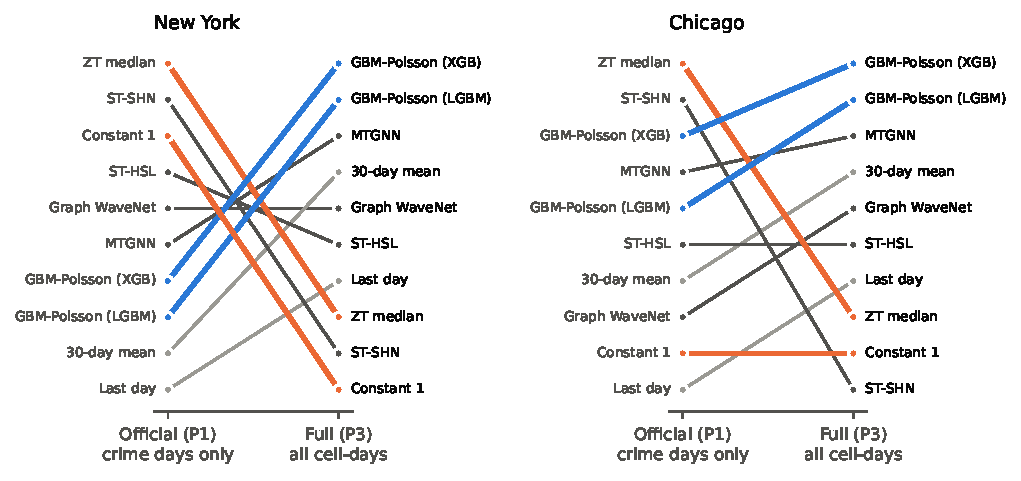
\includegraphics[width=\linewidth]{fig1_rank_change}
\caption{Ranks of the 10 models (ST-SHN validation-selected) under the official protocol P1 (mean MAE over crime cell-days) and the full protocol P3 (Poisson deviance over all cell-days). Blue: our gradient-boosted Poisson models; orange: the constant-1 and zero-truncated-median (ZT) predictors; dark gray: re-run deep models; light gray: naive forecasts. Rank 1 is best.}\label{fig:ranks}
\end{figure}

\begin{table}[t]\centering\small
\setlength{\tabcolsep}{4pt}\caption{The protocol decides the ranking. Mean MAE under the official protocol P1 and Poisson deviance under the full protocol P3 (all cell-days), with ranks among the 11 models (5 seeds for learned models). Kendall's $\tau$ between the two rankings: NYC $\tau=-0.45$ ($p=0.06$), CHI $\tau=0.00$ ($p=1.00$).}\label{tab:rankings}
\begin{tabular}{lrrrrrrrr}\toprule
 & \multicolumn{4}{c}{New York} & \multicolumn{4}{c}{Chicago}\\\cmidrule(lr){2-5}\cmidrule(lr){6-9}
Model & P1 MAE & rank & P3 dev. & rank & P1 MAE & rank & P3 dev. & rank\\\midrule
GBM-Poisson, XGBoost (ours) & 0.915 & 8 & 0.349 & 1 & 1.016 & 4 & 0.501 & 1 \\
GBM-Poisson, LightGBM (ours) & 0.920 & 9 & 0.350 & 2 & 1.022 & 6 & 0.502 & 2 \\
MTGNN & 0.912 & 7 & 0.361 & 3 & 1.019 & 5 & 0.515 & 3 \\
Graph WaveNet & 0.912 & 6 & 0.373 & 5 & 1.039 & 9 & 0.530 & 5 \\
30-day mean & 0.928 & 10 & 0.362 & 4 & 1.035 & 8 & 0.518 & 4 \\
ST-HSL & 0.894 & 5 & 0.480 & 6 & 1.023 & 7 & 0.632 & 6 \\
ST-SHN & 0.680 & 3 & 1.852 & 9 & 0.933 & 2 & 2.414 & 10 \\
Zero-truncated median (exploit) & 0.607 & 1 & 1.826 & 8 & 0.866 & 1 & 1.728 & 8 \\
Constant 1 & 0.806 & 4 & 1.951 & 11 & 1.330 & 10 & 2.262 & 9 \\
Last day & 1.236 & 11 & 0.931 & 7 & 1.429 & 11 & 1.468 & 7 \\
\bottomrule\end{tabular}\end{table}


\subsection{The decision protocol agrees with the full protocol, not with the official one}\label{sec:res-decision}
A planner who uses the forecast to choose the 10\,\% of cells to watch each day cares about the share of crime those cells capture. Table~\ref{tab:decision} reports this hit rate (post hoc). Our forecasters capture 67.7--67.8\,\% of crimes in New York and 51.4\,\% in Chicago in 10\,\% of the area (PAI 6.7 and 5.1), closely followed by MTGNN (67.5\,\%, 51.3\,\%) and the 30-day mean (67.5\,\%, 51.1\,\%). ST-SHN, second under P1, captures only 47.3\,\% and 36.2\,\%, with large variation over seeds, and the zero-truncated median 55.1\,\% and 49.0\,\%. The P4 ranking agrees almost perfectly with the P3 ranking ($\tau=0.96$ in New York, $0.87$ in Chicago, both $p<0.001$) and not with the P1 ranking ($\tau=-0.47$, $p=0.07$, and $0.29$, $p=0.29$). The official metric therefore misleads not only on a statistical loss but on the operational criterion used in place-based policing. Differences among the best models are small under P4: the protocol separates sound from unsound forecasts more than it separates sound forecasts from each other.

\begin{table}[t]\centering\small\setlength{\tabcolsep}{4pt}
\caption{Decision protocol P4 on the benchmark: share of each day's crimes that fall in the 10\,\% of cells with the highest forecast (hit rate), the Predictive Accuracy Index (PAI = hit rate / area share; 1 = no better than a random list), and the rank among the 10 models (mean over seeds). Kendall's $\tau$ of the P4 ranking with P3: NYC 0.96, CHI 0.87; with P1: NYC -0.47, CHI 0.29.}\label{tab:decision}
\begin{tabular}{lrrrrrr}\toprule
 & \multicolumn{3}{c}{New York} & \multicolumn{3}{c}{Chicago}\\\cmidrule(lr){2-4}\cmidrule(lr){5-7}
Model & Hit rate (\%) & PAI & Rank & Hit rate (\%) & PAI & Rank\\\midrule
GBM-Poisson, XGBoost (ours) & 67.7 & 6.67 & 2 & 51.4 & 5.08 & 1 \\
GBM-Poisson, LightGBM (ours) & 67.8 & 6.68 & 1 & 51.4 & 5.08 & 2 \\
MTGNN & 67.5 & 6.65 & 3 & 51.3 & 5.07 & 3 \\
30-day mean & 67.5 & 6.65 & 4 & 51.1 & 5.05 & 4 \\
ST-HSL & 66.7 & 6.57 & 6 & 51.0 & 5.04 & 5 \\
Graph WaveNet & 66.9 & 6.59 & 5 & 50.8 & 5.02 & 6 \\
Zero-truncated median & 55.1 & 5.42 & 8 & 49.0 & 4.84 & 7 \\
Last day & 55.6 & 5.47 & 7 & 44.2 & 4.37 & 8 \\
ST-SHN & 47.3 & 4.66 & 9 & 36.2 & 3.57 & 9 \\
Constant 1 & 10.2 & 1.00 & 10 & 10.1 & 1.00 & 10 \\
\bottomrule\end{tabular}\end{table}


\subsection{Gradient-boosted Poisson against deep models trained either way}\label{sec:res-simple}
In the literature setting, our forecaster has a lower P3 deviance than ST-HSL, ST-SHN, Graph WaveNet and MTGNN in both cities, and its worst seed is better than the best seed of each deep model (Supplementary Table~S3). The margins over MTGNN are small---0.349 vs.\ 0.361 in New York and 0.501 vs.\ 0.515 in Chicago, about 3\,\%---but consistent over test days: the day-block bootstrap interval of the difference excludes zero, and our forecaster has the lower deviance on 85 (New York) and 83 (Chicago) of the 92 test days (Table~\ref{tab:bootstrap}). Against Graph WaveNet it is better on 92 and 91 days, against ST-HSL and ST-SHN on all days. A 30-day mean is itself competitive under P3 (0.362 and 0.518), better than Graph WaveNet and ST-HSL.

\begin{table}[!htbp]\centering\small\setlength{\tabcolsep}{3.5pt}
\caption{Full-protocol Poisson deviance of each model minus that of our XGBoost-Poisson forecaster (both averaged over seeds), with a 95\,\% interval from a bootstrap over the 92 test days (2{,}000 resamples), and the number of test days on which our forecaster has the lower deviance. Positive = our forecaster is better.}\label{tab:bootstrap}
\begin{tabular}{lrrrrrr}\toprule
 & \multicolumn{3}{c}{New York} & \multicolumn{3}{c}{Chicago}\\\cmidrule(lr){2-4}\cmidrule(lr){5-7}
Compared with & Difference & 95\,\% CI & Days & Difference & 95\,\% CI & Days\\\midrule
MTGNN & 0.0121 & [0.0107, 0.0136] & 85/92 & 0.0137 & [0.0114, 0.0161] & 83/92 \\
Graph WaveNet & 0.0237 & [0.0217, 0.0256] & 92/92 & 0.0289 & [0.0263, 0.0314] & 91/92 \\
ST-HSL & 0.1312 & [0.1290, 0.1335] & 92/92 & 0.1308 & [0.1278, 0.1340] & 92/92 \\
ST-SHN & 1.5036 & [1.4970, 1.5106] & 92/92 & 1.9131 & [1.9011, 1.9242] & 92/92 \\
30-day mean & 0.0134 & [0.0115, 0.0153] & 86/92 & 0.0169 & [0.0142, 0.0195] & 84/92 \\
\bottomrule\end{tabular}\end{table}


Part of this gap could be due to the objective rather than the architecture, since the deep models were trained with squared error and selected on crime days. Table~\ref{tab:poisson} separates the two. Trained with the Poisson likelihood on all cell-days and selected on the validation deviance, both deep models improve on the full task: MTGNN from 0.361 to 0.353 in New York and from 0.515 to 0.508 in Chicago, Graph WaveNet from 0.373 to 0.362 and from 0.530 to 0.511. Our forecaster remains better than every Poisson-trained run, but the margin over MTGNN shrinks to 1.1\,\% and 1.4\,\%; the bootstrap interval of the difference still excludes zero, and our forecaster has the lower deviance on 74 and 72 of the 92 days. Under P4 the Poisson-trained MTGNN and our forecaster capture the same share of crime (67.7\,\% and 51.3--51.4\,\%). The same change of objective \emph{worsens} both deep models under the official protocol (P1 MAE 0.928 instead of 0.912 for MTGNN in New York; 0.942 instead of 0.912 for Graph WaveNet), because a model fitted to all cell-days predicts less crime on the days the official metric looks at: under P1, improving the forecast of the full task is penalised. The claim is therefore not that boosting is much better than the best deep model. It is that the deep-model advantage reported under P1 does not exist on the full task, whichever loss the deep models are trained with, and that a fair comparison needs the same objective on both sides.

\begin{table}[!htbp]\centering\scriptsize\setlength{\tabcolsep}{3pt}
\caption{Deep baselines trained in the literature setting (squared error, epoch chosen on crime days) and in the Poisson setting (Poisson likelihood on all cell-days, epoch chosen on the validation deviance, the rule of our forecaster); 5 seeds each. P1: mean MAE on crime cell-days; P3: Poisson deviance on all cell-days ($\pm$ sd over seeds); P4: hit rate of the daily top-10\,\% list; Moran's $I$ of the per-cell mean Pearson residual ($^{*}$ significant at 5\,\% in every seed); P3 deviance minus that of our forecaster with a 95\,\% day-block bootstrap interval, and the test days on which our forecaster is better.}\label{tab:poisson}
\begin{tabular}{llrrrrlr}\toprule
Model & Training & P1 MAE & P3 deviance & P4 hit (\%) & Moran's $I$ & P3 minus ours [95\,\% CI] & Days\\\midrule
\multicolumn{8}{l}{\textit{New York}}\\
GBM-Poisson (ours) & Poisson & 0.915 & 0.349\,{\tiny$\pm$0.000} & 67.7 & 0.01 & -- & -- \\
Graph WaveNet & Literature & 0.912 & 0.373\,{\tiny$\pm$0.002} & 66.9 & 0.40$^{*}$ & +0.0237 [+0.0217, +0.0256] & 92/92 \\
Graph WaveNet & Poisson & 0.942 & 0.362\,{\tiny$\pm$0.001} & 67.0 & -0.02 & +0.0128 [+0.0110, +0.0144] & 87/92 \\
MTGNN & Literature & 0.912 & 0.361\,{\tiny$\pm$0.005} & 67.5 & 0.33$^{*}$ & +0.0121 [+0.0107, +0.0136] & 85/92 \\
MTGNN & Poisson & 0.928 & 0.353\,{\tiny$\pm$0.000} & 67.7 & 0.08 & +0.0039 [+0.0027, +0.0051] & 74/92 \\
\midrule
\multicolumn{8}{l}{\textit{Chicago}}\\
GBM-Poisson (ours) & Poisson & 1.016 & 0.501\,{\tiny$\pm$0.000} & 51.4 & 0.06 & -- & -- \\
Graph WaveNet & Literature & 1.039 & 0.530\,{\tiny$\pm$0.003} & 50.8 & 0.27$^{*}$ & +0.0289 [+0.0263, +0.0315] & 91/92 \\
Graph WaveNet & Poisson & 1.031 & 0.511\,{\tiny$\pm$0.001} & 50.8 & 0.14 & +0.0106 [+0.0086, +0.0126] & 81/92 \\
MTGNN & Literature & 1.019 & 0.515\,{\tiny$\pm$0.003} & 51.3 & 0.37$^{*}$ & +0.0137 [+0.0114, +0.0162] & 83/92 \\
MTGNN & Poisson & 1.020 & 0.508\,{\tiny$\pm$0.002} & 51.3 & 0.12 & +0.0069 [+0.0051, +0.0089] & 72/92 \\
\bottomrule\end{tabular}\end{table}


\subsection{Spatial structure of the errors}\label{sec:res-spatial}
Figure~\ref{fig:residmaps} maps the mean residual of three models in both cities (post hoc). The residuals of our forecaster show no spatial pattern: their Moran's $I$ is 0.014 in New York and 0.063 in Chicago, and not significant in any of the five seeds ($p\ge0.14$; Supplementary Table~S7). The deep models in the literature setting leave clustered errors. MTGNN over-predicts in parts of the busiest districts of both cities and has $I=0.33$ (New York) and $0.37$ (Chicago), Graph WaveNet $0.40$ and $0.27$, all significant in every seed; ST-HSL is intermediate (0.23 and 0.09, significant in some seeds only). ST-SHN over-predicts almost everywhere ($I=0.43$ and $0.53$), the spatial footprint of its training on crime days only. A 30-day mean leaves the same kind of clustered error ($I=0.27$, $0.34$). The clustering is a property of the training objective, not of the architecture: trained with the Poisson loss on all cell-days, the same two networks have $I$ between $-0.02$ and $0.14$, significant in no city (Table~\ref{tab:poisson}). A plausible mechanism is the selection rule: choosing the epoch by its error on crime days favours epochs that predict too much crime, and the resulting over-prediction is largest, and therefore spatially organised, where crime is common. For evaluation the point is that a citywide difference of a few per cent between two models can hide systematic local over-prediction concentrated in a few districts, which only a map or a spatial statistic reveals.

\begin{figure}[t]\centering
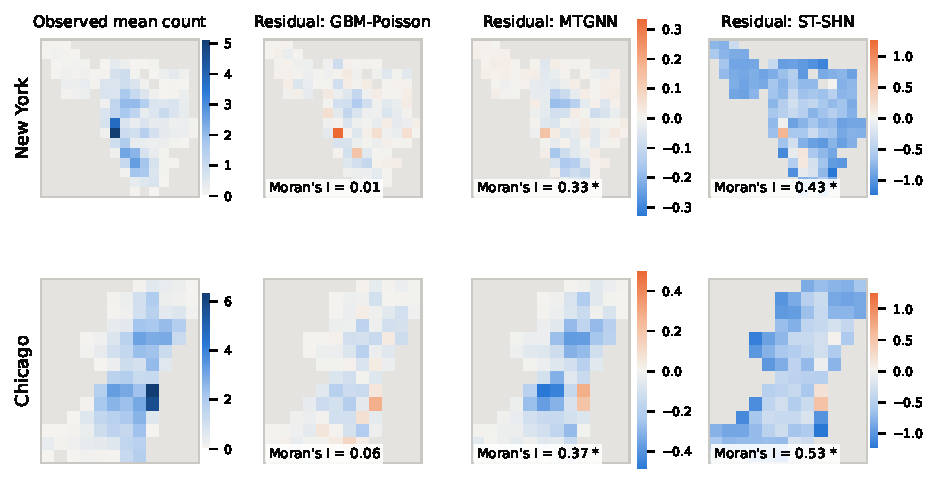
\includegraphics[width=\linewidth]{fig6_bench_residual_maps}
\caption{Benchmark grid, test period (post hoc). Left: observed mean count per cell-day (all categories). Right: mean residual (observed minus forecast; orange = under-prediction, blue = over-prediction) of our XGBoost-Poisson forecaster, MTGNN and ST-SHN (seed 0; GBM-Poisson and MTGNN share a colour scale, ST-SHN has its own). Gray: cells without any crime in the test period. Moran's $I$ of the mean Pearson residual, averaged over five seeds; $^*$ significant at 5\,\% in every seed. Cells are shown in the row and column order of the benchmark files.}\label{fig:residmaps}
\end{figure}

\subsection{The protocol effect depends on the spatial unit}\label{sec:res-scale}
Table~\ref{tab:scale} repeats the comparison on coarser cells (post hoc). Aggregation reduces the share of zero cell-days from 87\,\% to 70\,\% and 41\,\% in New York and from 74\,\% to 53\,\% in Chicago, and with it the disagreement between P1 and P3: Kendall's $\tau$ rises from $-0.42$ to $0.56$ at 6\,km and $0.78$ at 12\,km in New York, and from $0.16$ to $0.69$ in Chicago. The exploit does not disappear: the zero-truncated median is the best model under P1 at every scale and among the worst under P3, and a model trained on crime days only (ST-SHN) becomes far worse under P3 at coarse scales, because its over-prediction accumulates over the cells of a block. The full and decision protocols agree at every scale ($\tau\ge0.64$), and our forecaster is the best model under P3 at every scale. How strongly zero-masking distorts a comparison is thus a property of the spatial unit, which is why benchmark results at one grid size should not be read as statements about forecasting at the units on which agencies act.

\begin{table}[!htbp]\centering\small\setlength{\tabcolsep}{4pt}
\caption{Spatial scale. The benchmark's 3-km grid aggregated to 2$\times$2 blocks (about 6\,km) and, in New York, 4$\times$4 blocks (about 12\,km); daily counts, expected counts summed over the block, the constant-1 and zero-truncated-median predictors re-derived at each scale. Share of zero units, Kendall's $\tau$ between model rankings under the official protocol P1 and the full protocol P3 and between the decision protocol P4 and P3 (10 models; $^{*}$\,$p<0.05$), and the best model under P1 and P3.}\label{tab:scale}
\begin{tabular}{lrrrrll}\toprule
Scale & Units & Zero (\%) & $\tau$(P1, P3) & $\tau$(P4, P3) & Best under P1 & Best under P3\\\midrule
\multicolumn{7}{l}{\textit{New York}}\\
3 km (original) & 256 & 87 & -0.42 & +0.96$^{*}$ & ZT median & GBM-Poisson \\
6 km & 64 & 70 & +0.56$^{*}$ & +0.82$^{*}$ & ZT median & GBM-Poisson \\
12 km & 16 & 41 & +0.78$^{*}$ & +0.76$^{*}$ & ZT median & GBM-Poisson \\
\midrule
\multicolumn{7}{l}{\textit{Chicago}}\\
3 km (original) & 168 & 74 & +0.16 & +0.87$^{*}$ & ZT median & GBM-Poisson \\
6 km & 42 & 53 & +0.69$^{*}$ & +0.64$^{*}$ & ZT median & GBM-Poisson \\
\bottomrule\end{tabular}\end{table}


\subsection{The published state of the art is reproduced only with its official seed}\label{sec:res-repro}
Figure~\ref{fig:repro} compares published P1 numbers with our re-runs (per-cell values in Appendix Table~\ref{tab:repro}). Averaged over five seeds, ST-HSL is worse than published in all eight cells (mean $+5.3$\,\%), and the 95\,\% interval of the gap lies above zero in six of them (post hoc). The seed-level picture is more informative. In New York, the official seed 523 reproduces the published numbers ($-3.5$ to $+0.4$\,\% across categories), but each of the other four seeds is worse in every category, by 1.7 to 15.1\,\%: the published figures are consistent with a favourable draw from a wide seed distribution. In Chicago no seed reaches the published value in any category; the official seed is 1.0--12.6\,\% worse, and the largest gap is assault (published 0.667, five-seed mean $0.734\pm0.019$). Through the same pipeline, MTGNN reproduces its published numbers within $-2.4$ to $+2.0$\,\% and Graph WaveNet within $-0.1$ to $+3.4$\,\% in New York, but $+1.7$ to $+4.2$\,\% in Chicago. Part of the Chicago gap may therefore be common to our setup; the ST-HSL gap there is about twice that of the baselines. The published baseline numbers were produced by the ST-HSL authors under the same protocol, which makes them a fair reference.

\begin{figure}[t]\centering
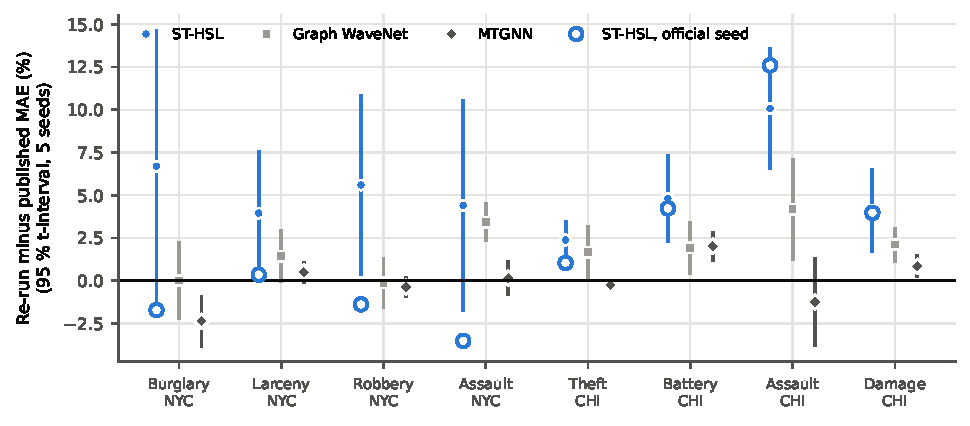
\includegraphics[width=\linewidth]{fig2_reproduction_gap}
\caption{Reproduction gap under the official protocol: re-run minus published MAE in per cent of the published value, with 95\,\% $t$-intervals over five seeds. Hollow circles: ST-HSL with its official seed (523) alone.}\label{fig:repro}
\end{figure}

ST-SHN behaves differently: its re-run is better than published in every cell (mean $-18.2$\,\%). The longer budget changes little (P1 MAE 0.713 vs.\ 0.710 in New York and 0.984 vs.\ 0.980 in Chicago for 10 vs.\ 25 epochs), and selecting the epoch on test or on validation MAPE gives practically identical results (Supplementary Table~S4). Choosing the reported epoch on the test set is unsound practice, but on this benchmark its optimism is negligible; ST-SHN's large P1 advantage comes from training on crime days only (Section~\ref{sec:res-exploit}).

\subsection{The protocol is current practice}\label{sec:res-census}
Table~\ref{tab:census} summarises the census. All six count-forecasting codebases score only non-zero cells in their test metric: ST-SHN and ST-HSL through explicit masks; CL4ST, STExplainer and EasyST through a shared metric module that drops cells with $y\le$ \texttt{mae\_thresh} $=0$; and ST-HHOL (ICLR 2026) through a masked MAE with \texttt{null\_val} $=0$, which it also uses as its training loss. The evidence is direct for four codebases; for CL4ST and STExplainer, which do not release a crime pipeline, it follows from the shared metric code and the shipped configuration. The one exception, HAGEN, is a classification model scored by F1 over all cells. The census also records two obstacles to replication: ST-HHOL does not release its data, and three of the codebases release no pipeline for the NYC/CHI benchmark on which they report crime results. This is why we could audit, but not re-run, the most recent models.

\begin{table}[!htbp]\centering\scriptsize
\caption{Protocol census of public crime-prediction code, audited automatically at pinned commits (Section~\ref{sec:census}). \emph{Indirect}: the crime pipeline was not released; the finding follows from the shared metric code and the shipped configuration.}\label{tab:census}
\setlength{\tabcolsep}{3pt}\begin{tabularx}{\linewidth}{@{}>{\raggedright\arraybackslash}p{1.45cm}>{\raggedright\arraybackslash}p{2.0cm}>{\raggedright\arraybackslash}p{1.25cm}>{\raggedright\arraybackslash}X>{\raggedright\arraybackslash}p{2.1cm}>{\raggedright\arraybackslash}p{1.8cm}>{\raggedright\arraybackslash}p{0.9cm}>{\raggedright\arraybackslash}p{1.05cm}@{}}\toprule
Code & Paper & Task & Cells scored by the test metric & Training loss & Epoch reported & Zeros ignored & Evidence\\\midrule
CL4ST & Tang et al., CIKM 2023 & regression & cells with y $>$ 0 when mae\_thresh = 0.0 (shipped config) & smooth L1 on all cells & validation & yes & indirect \\
EasyST & Tang et al., CIKM 2024 & regression & cells with y $>$ 0 when mae\_thresh = 0.0 (shipped config) & MSE on all cells & -- & yes & direct \\
HAGEN & Wang et al., HAGEN (crime occurrence) & classification & all cells (macro/micro F1 of occurrence) & binary cross-entropy on all cells & best validation F1 & no & direct \\
ST-HHOL & ST-HHOL, ICLR 2026 & regression & cells with y $\neq$ 0 (null\_val = 0) & masked MAE: crime cells only & validation & yes & direct \\
ST-HSL & Li et al., ICDE 2022 & regression & crime cell-days only (y $>$ 0) & all cell-days & best validation RMSE + MAE & yes & direct \\
ST-SHN & Xia et al., IJCAI 2021 & regression & crime cell-days only (y $>$ 0), and only cells active on 20--80 \% of days & crime cell-days only & best TEST MAPE & yes & direct \\
STExplainer & Tang et al., STExplainer & regression & cells with y $>$ 0 when mae\_thresh = 0.0 (shipped config) & -- & validation & yes & indirect \\
\bottomrule\end{tabularx}\end{table}


\subsection{Weekly forecasts at planning units}\label{sec:res-weekly}
Table~\ref{tab:weekly} reports test deviances for the weekly panels. LightGBM-Poisson, the GRU and the ST-GRU are statistically indistinguishable: their deviance differences lie between $-0.016$ and $+0.037$ and none is significant in every seed. XGBoost-Poisson is close behind (significantly worse only in New York), and the Poisson GLM is clearly worse, by 0.05--0.16. The selected forecaster beats every naive and statistical baseline at every horizon in every city and seed (60 of 60 comparisons significant), for example by 0.10--0.12 deviance over exponential smoothing at $H=1$. Graph-diffusion input does not improve on the plain GRU at the area level: community areas and precincts are large enough that a neighbour's recent counts add little to an area's own history and to the city-wide type totals that every model already sees. At the area level the forecaster's mean residuals are spatially clustered in Chicago ($I=0.33$, $p=0.001$) and San Francisco ($0.27$, $p=0.006$) but not in New York ($-0.04$; Supplementary Table~S12): neighbouring community areas share under- or over-prediction over the test year, a reminder that a forecast that is unbiased citywide can be biased for districts. On current data, a well-specified boosted Poisson model matches the neural forecasters at a fraction of the computational cost.

\begin{table}[!htbp]\centering\scriptsize\setlength{\tabcolsep}{3.5pt}
\caption{Weekly area $\times$ crime-type forecasts, test period (July 2024 onwards): mean Poisson deviance (lower is better; $\pm$ sd over 3 seeds for learned models) at horizons of 1 and 4 weeks. The forecaster selected on validation deviance is LightGBM-Poisson.}\label{tab:weekly}
\begin{tabular}{lrrrrrr}\toprule
 & \multicolumn{3}{c}{$H=1$} & \multicolumn{3}{c}{$H=4$}\\\cmidrule(lr){2-4}\cmidrule(lr){5-7}
Model & Chicago & New York & San Francisco & Chicago & New York & San Francisco\\\midrule
LightGBM-Poisson & 1.283\,{\tiny$\pm$0.001} & 1.420\,{\tiny$\pm$0.002} & 1.180\,{\tiny$\pm$0.004} & 1.326\,{\tiny$\pm$0.001} & 1.502\,{\tiny$\pm$0.001} & 1.240\,{\tiny$\pm$0.004} \\
XGBoost-Poisson & 1.285\,{\tiny$\pm$0.001} & 1.435\,{\tiny$\pm$0.002} & 1.188\,{\tiny$\pm$0.005} & 1.326\,{\tiny$\pm$0.002} & 1.519\,{\tiny$\pm$0.003} & 1.248\,{\tiny$\pm$0.006} \\
GRU (global) & 1.278\,{\tiny$\pm$0.004} & 1.422\,{\tiny$\pm$0.004} & 1.178\,{\tiny$\pm$0.006} & 1.322\,{\tiny$\pm$0.001} & 1.514\,{\tiny$\pm$0.034} & 1.227\,{\tiny$\pm$0.010} \\
ST-GRU (graph diffusion input) & 1.281\,{\tiny$\pm$0.006} & 1.432\,{\tiny$\pm$0.005} & 1.179\,{\tiny$\pm$0.007} & 1.321\,{\tiny$\pm$0.011} & 1.539\,{\tiny$\pm$0.037} & 1.224\,{\tiny$\pm$0.015} \\
Poisson GLM & 1.363\,{\tiny$\pm$0.002} & 1.484\,{\tiny$\pm$0.002} & 1.337\,{\tiny$\pm$0.009} & 1.393\,{\tiny$\pm$0.003} & 1.552\,{\tiny$\pm$0.001} & 1.385\,{\tiny$\pm$0.004} \\
Historical average (52 w) & 1.360 & 1.535 & 1.252 & 1.376 & 1.563 & 1.275 \\
Exp. smoothing (0.3) & 1.405 & 1.522 & 1.282 & 1.470 & 1.626 & 1.323 \\
Moving average (4 w) & 1.515 & 1.636 & 1.395 & 1.583 & 1.744 & 1.432 \\
Last week & 2.688 & 2.872 & 2.405 & 2.795 & 3.067 & 2.484 \\
Seasonal naive (52 w) & 2.964 & 3.395 & 2.686 & 2.964 & 3.395 & 2.686 \\
\bottomrule\end{tabular}\end{table}


\subsection{Interval calibration by series volume and by area}\label{sec:res-intervals}
Figure~\ref{fig:coverage} and Table~\ref{tab:intervals} show coverage by volume quintile at $H=1$. Every method reaches about 90\,\% coverage overall, but the Poisson and split-conformal intervals do so by over-covering quiet series and under-covering busy ones: split CP covers 84.3\,\% (Chicago), 83.1\,\% (New York) and 78.9\,\% (San Francisco) of the busiest quintile, Poisson intervals 87.7\,\%, 82.5\,\% and 85.5\,\%. A single global calibration, or a Poisson assumption, fits the many quiet series and leaves the busy, over-dispersed ones under-covered. Mondrian CP removes this pattern: every quintile in Chicago and New York lies within 2.0 points of 90\,\% at every horizon, and over all cities and horizons its worst under-coverage is 0.9 points (post hoc criterion; 1.2 points in the third stage). The pre-specified criterion---all quintiles within 3 points---fails only because the quietest San Francisco quintile is over-covered by 5.1 points: 40\,\% of its series-weeks are zero, and an integer interval around a forecast close to zero cannot be narrower than $[0,0]$ or $[0,1]$. CQR is competitive at $H=1$ but less stable over time (Section~\ref{sec:res-rolling}).

\begin{figure}[t]\centering
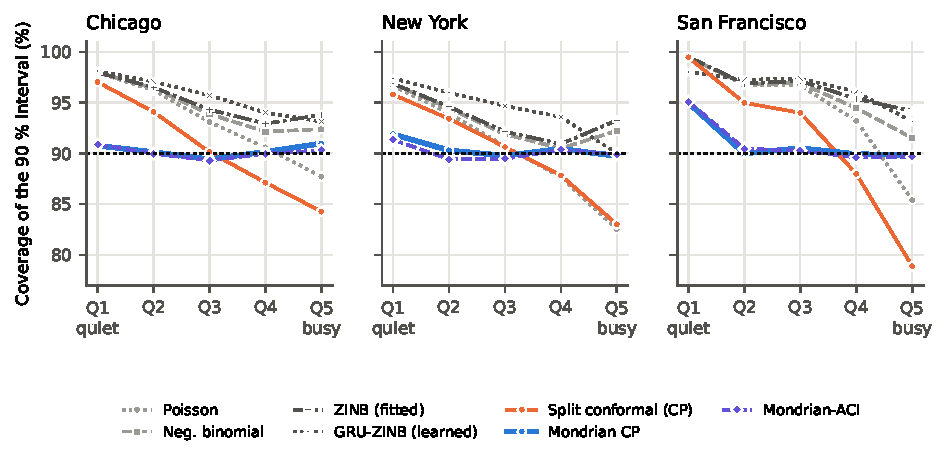
\includegraphics[width=\linewidth]{fig3_coverage_by_quintile}
\caption{Coverage of 90\,\% intervals by series-volume quintile ($H=1$, test period, seed 0; third stage, which includes the zero-inflated baselines and matches the first stage within 0.2 points).}\label{fig:coverage}
\end{figure}

\begin{table*}[t]\centering\scriptsize\setlength{\tabcolsep}{3.5pt}
\caption{90\,\% intervals around the LightGBM-Poisson forecast, $H=1$, test period, seed 0. Coverage overall and per series-volume quintile (Q1 quietest, Q5 busiest), mean width, mean interval score \citep{gneiting2007strictly} (lower is better) and the worst under-coverage over the quintiles (points below 90\,\%; negative = no quintile under-covers).}\label{tab:intervals}
\begin{tabular}{lrrrrrrrrr}\toprule
Method & Coverage & Width & Int.\ score & Q1 & Q2 & Q3 & Q4 & Q5 & Worst under\\\midrule
\multicolumn{10}{l}{\textit{Chicago}}\\
Poisson & 93.1 & 6.23 & 9.26 & 97.9 & 96.2 & 93.1 & 90.5 & 87.7 & 2.3 \\
Neg. binomial & 94.6 & 6.93 & 9.13 & 97.9 & 96.4 & 93.9 & 92.1 & 92.5 & -2.1 \\
Split conformal (CP) & 90.6 & 5.55 & 9.69 & 97.0 & 94.1 & 90.2 & 87.2 & 84.3 & 5.7 \\
Locally weighted CP & 90.5 & 6.26 & 10.16 & 91.4 & 92.2 & 90.9 & 89.6 & 88.3 & 1.7 \\
CQR & 90.2 & 6.30 & 9.66 & 91.5 & 89.8 & 89.2 & 89.6 & 90.8 & 0.8 \\
ACI & 90.1 & 5.47 & 9.77 & 96.9 & 93.8 & 89.7 & 86.5 & 83.7 & 6.3 \\
Mondrian CP & 90.3 & 6.01 & 9.67 & 90.8 & 90.0 & 89.6 & 90.2 & 90.8 & 0.4 \\
Mondrian-ACI & 90.1 & 5.93 & 9.69 & 90.9 & 89.9 & 89.4 & 89.9 & 90.3 & 0.6 \\
\midrule
\multicolumn{10}{l}{\textit{New York}}\\
Poisson & 90.3 & 9.55 & 15.38 & 96.6 & 93.9 & 90.7 & 87.7 & 82.5 & 7.5 \\
Neg. binomial & 93.2 & 11.33 & 14.69 & 96.8 & 94.5 & 91.8 & 90.6 & 92.2 & -0.6 \\
Split conformal (CP) & 90.1 & 9.46 & 15.39 & 95.8 & 93.3 & 90.6 & 87.8 & 83.1 & 6.9 \\
Locally weighted CP & 90.4 & 10.95 & 16.75 & 93.4 & 92.8 & 91.7 & 88.7 & 85.2 & 4.8 \\
CQR & 90.0 & 10.76 & 15.35 & 91.4 & 89.4 & 89.5 & 90.9 & 88.9 & 1.1 \\
ACI & 90.0 & 9.43 & 15.41 & 95.7 & 93.3 & 90.5 & 87.6 & 82.9 & 7.1 \\
Mondrian CP & 90.5 & 10.29 & 15.04 & 91.9 & 90.3 & 89.8 & 90.5 & 89.8 & 0.2 \\
Mondrian-ACI & 90.1 & 10.26 & 15.09 & 91.3 & 89.4 & 89.5 & 90.4 & 89.9 & 0.6 \\
\midrule
\multicolumn{10}{l}{\textit{San Francisco}}\\
Poisson & 94.3 & 4.56 & 7.51 & 99.5 & 96.7 & 96.7 & 93.3 & 85.5 & 4.5 \\
Neg. binomial & 95.8 & 5.30 & 7.06 & 99.5 & 96.8 & 96.9 & 94.4 & 91.5 & -1.5 \\
Split conformal (CP) & 91.1 & 3.83 & 8.21 & 99.5 & 94.9 & 93.9 & 88.1 & 78.9 & 11.1 \\
Locally weighted CP & 90.8 & 4.23 & 8.02 & 95.0 & 91.2 & 92.7 & 89.2 & 85.9 & 4.1 \\
CQR & 91.1 & 4.73 & 7.71 & 96.2 & 90.2 & 89.5 & 89.4 & 90.0 & 0.6 \\
ACI & 90.3 & 3.70 & 8.41 & 99.5 & 94.7 & 93.4 & 86.5 & 77.4 & 12.6 \\
Mondrian CP & 91.1 & 4.23 & 7.72 & 95.1 & 90.2 & 90.5 & 89.7 & 89.9 & 0.3 \\
Mondrian-ACI & 91.0 & 4.22 & 7.73 & 95.1 & 90.5 & 90.3 & 89.5 & 89.8 & 0.5 \\
\bottomrule\end{tabular}\end{table*}


Figure~\ref{fig:areamaps} maps the coverage of each area (post hoc). With split CP the worst area is covered 82.7\,\% (Chicago), 84.8\,\% (New York) and 77.0\,\% (San Francisco) of the weeks, 6.5\,\%, 1.3\,\% and 9.8\,\% of areas fall below 85\,\%, and coverage is spatially clustered ($I=0.34$, $0.13$ and $0.42$, all $p<0.05$): under-covered areas form contiguous districts---the Loop, the Near North and Near West Sides and the West Side (Austin, Humboldt Park, West Town) in Chicago, and the Mission, the Tenderloin and South of Market in San Francisco---while quiet peripheral areas are over-covered. With Mondrian CP no area falls below 86.4\,\%, 87.0\,\% and 86.4\,\%, and the clustering of coverage disappears in Chicago ($I=0.10$, $p=0.07$) and New York ($-0.08$) and is weaker in San Francisco ($0.26$, $p=0.01$), where large parks and the Presidio remain over-covered (Supplementary Table~S12). Calibration by forecast volume therefore also gives more uniform calibration across space, although it is not designed for it.

\begin{figure}[t]\centering
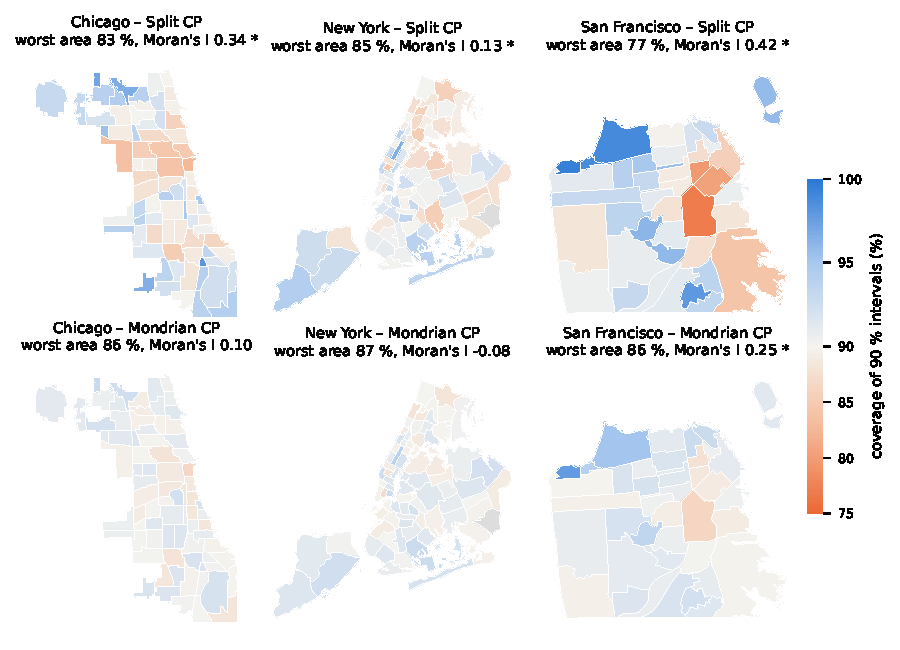
\includegraphics[width=\linewidth]{fig7_area_coverage_maps}
\caption{Coverage of 90\,\% intervals by area, split CP (top) and Mondrian CP (bottom) ($H=1$, test period, seed 0; post hoc). Orange: under-covered, blue: over-covered; gray: area not in the panel. Moran's $I$ of area coverage with queen contiguity; $^*$ $p<0.05$ (999 permutations).}\label{fig:areamaps}
\end{figure}

\paragraph{Zero-inflated intervals} Table~\ref{tab:zinb} adds the three zero-inflated baselines. The fitted zero-inflation is essentially zero in every city ($\hat\pi\le0.001$ globally and $\le0.009$ in any volume bin): once the forecast mean captures the many quiet series, the zeros are explained by the mean, and the ZINB reduces to the negative binomial. The learned GRU-ZINB is an equally good point forecaster (test deviance 1.280 vs.\ 1.284 for LightGBM in Chicago, 1.426 vs.\ 1.422 in New York, 1.177 vs.\ 1.186 in San Francisco) and learns a small zero-inflation (mean $\pi\approx0.06$). None of the three under-covers any volume quintile, but all over-cover by 7--10 points: overall coverage is 94--97\,\%, and the intervals are 14--37\,\% wider than Mondrian CP (mean width 7.24 vs.\ 6.01 in Chicago, 11.67 vs.\ 10.28 in New York, 5.82 vs.\ 4.24 in San Francisco for the fitted ZINB). Their interval score is nonetheless 3--9\,\% lower (better) than Mondrian's in every city, contrary to our pre-specified expectation. The reason is discreteness: for small counts the 5--95\,\% interval of a well-specified predictive distribution covers more than 90\,\% of outcomes, and the interval score, which is minimised by the true quantiles, rewards it; Mondrian reaches 90\,\% by rounding inward, which costs score when it misses. The second pre-specified expectation holds---Mondrian's worst under-coverage is 1.2 points and every zero-inflated baseline misses 90\,\% by more than 3 points in some quintile---but those misses are over-coverage, not under-coverage.

The choice between the two families is therefore one of guarantee. Mondrian gives nominal coverage, with the narrowest intervals, in every volume group; a well-dispersed negative binomial gives conservative coverage and a slightly better proper score; zero-inflation adds nothing over the negative binomial when the forecast mean is good. On the daily benchmark the same pattern holds: the fitted ZINB coincides with the NB (98.7--99.0\,\% coverage), while Mondrian covers 95.6--95.9\,\%---most test cell-days are zeros predicted near zero, which any interval containing 0 covers---with intervals about half as wide (1.03 vs.\ 1.52 in Chicago, 0.41 vs.\ 0.78 in New York; Supplementary Table~S5).

\begin{table}[t]\centering\scriptsize\setlength{\tabcolsep}{3.5pt}
\caption{Zero-inflated baselines (third run; $H=1$, seed 0). Overall coverage, mean width, mean interval score (lower is better), worst under- and over-coverage over the volume quintiles (points) and coverage of the busiest quintile Q5. $\hat\pi$: zero-inflation fitted on the calibration block.}\label{tab:zinb}
\begin{tabular}{lrrrrrr}\toprule
Method & Coverage & Width & Int.\ score & Worst under & Worst over & Q5\\\midrule
\multicolumn{7}{l}{\textit{Chicago} (fitted zero-inflation $\hat\pi=0.001$)}\\
Poisson & 93.1 & 6.24 & 9.27 & 2.3 & 7.9 & 87.7 \\
Neg. binomial & 94.6 & 6.93 & 9.14 & -2.1 & 8.0 & 92.4 \\
ZINB (fitted) & 95.1 & 7.24 & 9.20 & -2.9 & 8.0 & 93.8 \\
ZINB (fitted per volume bin) & 95.5 & 7.23 & 9.13 & -2.8 & 8.0 & 92.8 \\
GRU-ZINB (learned) & 95.6 & 7.17 & 9.06 & -3.1 & 8.1 & 93.1 \\
Split conformal (CP) & 90.5 & 5.54 & 9.69 & 5.7 & 7.0 & 84.3 \\
CQR & 90.8 & 6.35 & 9.56 & 1.0 & 3.8 & 91.0 \\
Mondrian CP & 90.3 & 6.01 & 9.67 & 0.6 & 1.0 & 91.0 \\
Mondrian-ACI & 90.1 & 5.93 & 9.69 & 0.7 & 0.9 & 90.3 \\
\midrule
\multicolumn{7}{l}{\textit{New York} (fitted zero-inflation $\hat\pi=0.000$)}\\
Poisson & 90.3 & 9.55 & 15.38 & 7.5 & 6.7 & 82.5 \\
Neg. binomial & 93.2 & 11.34 & 14.69 & -0.5 & 6.8 & 92.2 \\
ZINB (fitted) & 93.6 & 11.67 & 14.75 & -0.9 & 6.9 & 93.3 \\
ZINB (fitted per volume bin) & 94.3 & 11.61 & 14.64 & -1.3 & 7.6 & 91.3 \\
GRU-ZINB (learned) & 94.3 & 11.40 & 14.89 & 0.0 & 7.4 & 90.0 \\
Split conformal (CP) & 90.1 & 9.45 & 15.39 & 7.0 & 5.8 & 83.0 \\
CQR & 90.2 & 10.86 & 15.42 & 1.0 & 2.1 & 89.0 \\
Mondrian CP & 90.4 & 10.28 & 15.04 & 0.3 & 1.9 & 89.7 \\
Mondrian-ACI & 90.1 & 10.26 & 15.09 & 0.6 & 1.3 & 89.9 \\
\midrule
\multicolumn{7}{l}{\textit{San Francisco} (fitted zero-inflation $\hat\pi=0.000$)}\\
Poisson & 94.3 & 4.56 & 7.52 & 4.6 & 9.5 & 85.4 \\
Neg. binomial & 95.8 & 5.30 & 7.07 & -1.5 & 9.5 & 91.5 \\
ZINB (fitted) & 96.6 & 5.82 & 7.20 & -4.2 & 9.5 & 94.2 \\
ZINB (fitted per volume bin) & 96.9 & 5.80 & 7.14 & -3.5 & 9.5 & 93.5 \\
GRU-ZINB (learned) & 96.4 & 5.33 & 7.00 & -3.1 & 8.0 & 93.1 \\
Split conformal (CP) & 91.1 & 3.84 & 8.22 & 11.1 & 9.5 & 78.9 \\
CQR & 91.9 & 4.78 & 7.56 & 0.5 & 6.4 & 90.0 \\
Mondrian CP & 91.1 & 4.23 & 7.72 & 0.2 & 5.0 & 89.8 \\
Mondrian-ACI & 91.0 & 4.22 & 7.73 & 0.4 & 5.1 & 89.7 \\
\bottomrule\end{tabular}\end{table}


\subsection{Calibration over time and under the 2020 shift}\label{sec:res-rolling}
Table~\ref{tab:rolling} and Figure~\ref{fig:rolling} give the worst-quintile deviation for each rolling test year. In 2020, split CP deviates by 12.3 (Chicago) and 9.8 points (New York) and plain Mondrian by 4.0 and 4.5 points, mostly by under-covering as crime levels shifted. Mondrian-ACI, which adapts each bin's level week by week, stays within 1.3 points in 2020 and within 1.9 points in every year in both cities (post hoc). Global ACI restores overall coverage (89.4--89.5\,\% in 2020) but not coverage by volume (worst deviation 8.0--10.6 points), because a single level cannot correct errors of opposite sign in quiet and busy series. In San Francisco, from 2021, the Mondrian variants deviate by 4.1--4.8 points, again by over-covering the quietest quintile.

\begin{figure}[t]\centering
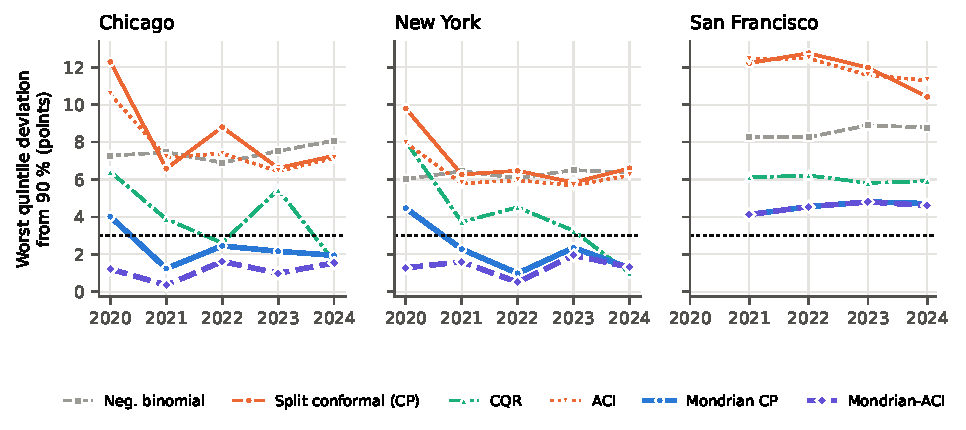
\includegraphics[width=\linewidth]{fig4_rolling_origins}
\caption{Worst deviation from 90\,\% coverage over the five volume quintiles, per rolling test year ($H=1$). Dotted line: the 3-point threshold fixed before the first run.}\label{fig:rolling}
\end{figure}

\begin{table}[!htbp]\centering\scriptsize\setlength{\tabcolsep}{3.5pt}
\caption{Rolling origins: worst deviation from 90\,\% coverage over the five series-volume quintiles (points), per test year ($H=1$). San Francisco starts in 2018, so its first test year is 2021.}\label{tab:rolling}
\begin{tabular}{l*{14}{r}}\toprule
 & \multicolumn{5}{c}{Chicago} & \multicolumn{5}{c}{New York} & \multicolumn{4}{c}{San Francisco}\\
Method & 2020 & 2021 & 2022 & 2023 & 2024 & 2020 & 2021 & 2022 & 2023 & 2024 & 2021 & 2022 & 2023 & 2024\\\midrule
Poisson & 7.7 & 7.4 & 6.7 & 7.3 & 8.0 & 9.9 & 7.1 & 7.3 & 6.5 & 6.7 & 9.4 & 8.3 & 8.9 & 8.8 \\
Neg. binomial & 7.3 & 7.5 & 6.9 & 7.5 & 8.1 & 6.0 & 6.4 & 6.1 & 6.5 & 6.4 & 8.3 & 8.3 & 8.9 & 8.8 \\
Split conformal (CP) & 12.3 & 6.6 & 8.8 & 6.6 & 7.3 & 9.8 & 6.3 & 6.5 & 5.8 & 6.6 & 12.2 & 12.8 & 12.0 & 10.4 \\
CQR & 6.4 & 3.9 & 2.6 & 5.5 & 1.6 & 8.0 & 3.7 & 4.5 & 3.3 & 1.0 & 6.1 & 6.2 & 5.8 & 5.9 \\
ACI & 10.6 & 7.2 & 7.4 & 6.4 & 7.1 & 8.0 & 5.8 & 6.0 & 5.7 & 6.2 & 12.4 & 12.5 & 11.6 & 11.3 \\
Mondrian CP & 4.0 & 1.2 & 2.4 & 2.2 & 1.9 & 4.5 & 2.3 & 1.0 & 2.4 & 1.3 & 4.1 & 4.5 & 4.8 & 4.7 \\
Mondrian-ACI & 1.2 & 0.4 & 1.6 & 1.0 & 1.5 & 1.3 & 1.6 & 0.5 & 1.9 & 1.3 & 4.1 & 4.5 & 4.8 & 4.6 \\
\bottomrule\end{tabular}\end{table}


Under the 2020 shift (Table~\ref{tab:shift}) the zero-inflated intervals, calibrated on pre-shift data, under-cover the busiest series by 1.9--3.5 points while still over-covering the quiet ones; their worst-quintile deviation is 6.1--7.8 points, against 1.1 (Chicago) and 1.3 (New York) for Mondrian-ACI. The learned GRU-ZINB under-covers least among the parametric methods ($-1.2$ and $0.6$ points) and again has the lowest interval score, at 93--95\,\% coverage.

\begin{table}[t]\centering\scriptsize\setlength{\tabcolsep}{3.5pt}
\caption{The 2020 test year (rolling origin, $H=1$; third run). Overall coverage, worst under-coverage and worst absolute deviation over the volume quintiles (points), and mean interval score.}\label{tab:shift}
\begin{tabular}{lrrrrrrrr}\toprule
 & \multicolumn{4}{c}{Chicago} & \multicolumn{4}{c}{New York}\\\cmidrule(lr){2-5}\cmidrule(lr){6-9}
Method & Cov. & Under & Worst & IS & Cov. & Under & Worst & IS\\\midrule
Poisson & 91.6 & 7.5 & 7.5 & 10.65 & 89.0 & 9.9 & 9.9 & 15.56 \\
Neg. binomial & 93.4 & 1.6 & 7.4 & 10.17 & 91.2 & 4.3 & 6.1 & 14.76 \\
ZINB (fitted) & 93.3 & 1.9 & 7.4 & 10.18 & 91.8 & 3.5 & 6.1 & 14.66 \\
ZINB (fitted per volume bin) & 93.7 & 2.5 & 7.8 & 10.19 & 92.7 & 3.4 & 6.7 & 14.62 \\
GRU-ZINB (learned) & 94.8 & -1.2 & 7.5 & 9.54 & 93.2 & 0.6 & 6.7 & 14.00 \\
Split conformal (CP) & 88.4 & 12.4 & 12.4 & 11.35 & 88.0 & 10.1 & 10.1 & 15.79 \\
CQR & 87.6 & 6.1 & 6.1 & 11.36 & 87.2 & 7.9 & 7.9 & 15.49 \\
Mondrian CP & 88.4 & 3.9 & 3.9 & 10.95 & 88.4 & 4.4 & 4.4 & 15.32 \\
Mondrian-ACI & 89.5 & 1.1 & 1.1 & 10.71 & 89.5 & 1.3 & 1.3 & 15.07 \\
\bottomrule\end{tabular}\end{table}


\subsection{Equity across communities}\label{sec:res-equity}
Table~\ref{tab:equity} and Figure~\ref{fig:equity} compare coverage in the poorest and richest thirds of areas. Mondrian CP covers 90.1--90.3\,\% in the poorest areas of all three cities, with gaps of $+0.1$, $-0.6$ and $-1.7$ points; the last is driven by over-coverage of rich San Francisco areas, not by under-coverage of poor ones. Split CP under-covers poor areas (89.3\,\%, 89.4\,\%, 88.6\,\%), with gaps up to $-4.8$ points, because poorer areas have higher counts and fall in the under-covered busy quintiles. Mondrian has a smaller poverty gap than split CP in every city. In New York a weak association between an area's coverage and its minority share remains ($\rho=-0.32$, $p=0.005$; split CP $\rho=-0.56$). Forecast skill over the four-week mean is similar across groups (0.21--0.24 deviance, with overlapping intervals). Top-10 risk lists give the poorest third of areas slightly more of the list slots than of the true top places (49\,\% vs.\ 46\,\% in Chicago, 50\,\% vs.\ 48\,\% in New York, 58\,\% vs.\ 57\,\% in San Francisco), and in Chicago the lists are less precise in poor areas (precision 0.57 vs.\ 0.74--0.83), i.e.\ they raise more false alarms there. These comparisons involve 40--77 areas per city and several groupings; they are descriptive, ecological, and do not establish causes.

\begin{figure}[t]\centering
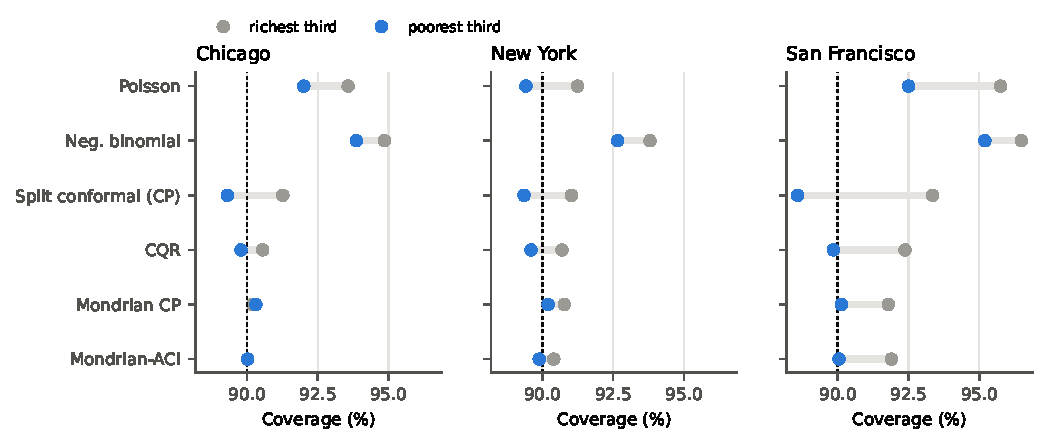
\includegraphics[width=\linewidth]{fig5_equity}
\caption{Coverage of 90\,\% intervals in the poorest (blue) and richest (gray) thirds of areas by ACS poverty rate ($H=1$, test).}\label{fig:equity}
\end{figure}

\begin{table}[!htbp]\centering\scriptsize\setlength{\tabcolsep}{3.5pt}
\caption{Equity of interval coverage ($H=1$, test). Coverage in the poorest third of areas (ACS 2022 poverty rate), the coverage gap poorest minus richest third (points), and Spearman's $\rho$ between an area's coverage and its minority share (77, 76 and 40 areas).}\label{tab:equity}
\begin{tabular}{lrrrrrrrrr}\toprule
 & \multicolumn{3}{c}{Chicago} & \multicolumn{3}{c}{New York} & \multicolumn{3}{c}{San Francisco}\\\cmidrule(lr){2-4}\cmidrule(lr){5-7}\cmidrule(lr){8-10}
Method & Cov.\ poor & Gap & $\rho$ minority & Cov.\ poor & Gap & $\rho$ minority & Cov.\ poor & Gap & $\rho$ minority\\\midrule
Poisson & 92.0 & -1.6 & -0.09 & 89.4 & -1.8 & -0.56 & 92.5 & -3.2 & -0.16 \\
Neg. binomial & 93.9 & -1.0 & -0.04 & 92.7 & -1.1 & -0.47 & 95.2 & -1.3 & -0.12 \\
Split conformal (CP) & 89.3 & -2.0 & -0.11 & 89.4 & -1.7 & -0.56 & 88.6 & -4.8 & -0.17 \\
CQR & 89.8 & -0.8 & -0.25 & 89.6 & -1.1 & -0.33 & 89.8 & -2.5 & -0.22 \\
Mondrian CP & 90.3 & +0.1 & +0.05 & 90.2 & -0.6 & -0.32 & 90.1 & -1.7 & -0.15 \\
Mondrian-ACI & 90.0 & -0.0 & +0.05 & 89.9 & -0.5 & -0.26 & 90.0 & -1.9 & -0.18 \\
\bottomrule\end{tabular}\end{table}


%% ===================================================================================
\section{Discussion}\label{sec:discussion}

\subsection{What the benchmark measures}
The official crime-prediction metric answers the question ``given that crime occurred here today, how many crimes were there?''. That is a legitimate question, but it is not forecasting: the conditioning event is the outcome being forecast. Optimising for it favours models that rarely predict low counts, and the rankings it produces are unrelated to, or the reverse of, rankings on the full task and on the hot-spot criterion used in place-based policing. The finding does not depend on a particular model. It follows from the metric, it is reproduced by two trivial predictors, it persists at coarser cells, and it is shared by every count-forecasting codebase in our census, including recent ones. Claims of state-of-the-art crime prediction made under this protocol should therefore be read as claims about a different task, and comparisons with them should be re-scored on all cell-days before conclusions are drawn.

The seed-level reproduction result points to a second, independent problem. A single run with a fixed seed is a draw from a distribution whose spread---up to 15\,\% of MAE on this benchmark---is larger than most of the improvements that the literature reports between successive models. Reporting several seeds with their spread would make such comparisons interpretable.

\subsection{Implications for planning and policing practice}
For an agency or a city analyst who considers a forecasting tool, the results translate into four questions to ask of any reported accuracy. \emph{Over which units and periods was it computed?} An accuracy figure computed only where crime occurred says nothing about how often the tool sends resources to places where nothing happens, which is where most of its recommendations will fall. \emph{At which spatial unit?} The same models rank differently on 3-km and on 12-km cells, so accuracy established on a research grid does not transfer to beats, precincts or neighbourhoods without being re-measured there. \emph{Where are the errors?} Two forecasts with nearly the same citywide error can differ in whether they systematically over-predict a few central districts---the pattern that, if acted on, concentrates attention where it is least needed and that, with recorded crime, can feed back into the data \citep{ensign2018runaway}. \emph{For whom does the uncertainty hold?} A tool whose 90\,\% intervals are correct on average but too narrow for the busiest places understates risk exactly where most decisions are made; volume-conditional calibration fixes this at no cost in average width. None of these checks requires a better model, only a different evaluation, and all of them can be run on the outputs a vendor or a research group already produces.

The weekly results also bear on the choice of model. At the planning units of three large cities, a gradient-boosted Poisson model on lagged counts matched recurrent and graph neural networks; it needs no GPU and can be re-trained and inspected by an analyst. Complex models may well add value with richer inputs, finer units or longer horizons than we studied; our results show only that the evidence for such gains must come from a full-task evaluation.

\subsection{A protocol for sparse urban count forecasts}\label{sec:protocol}
We suggest five rules for evaluating forecasts of sparse urban counts.
\begin{enumerate}[leftmargin=*,itemsep=2pt]
\item \textbf{Score all space-time units.} Use a proper loss for counts---Poisson deviance, or a proper score for the predictive distribution \citep{czado2009predictive}---and add the decision criterion the forecast serves, such as the hit rate or PAI of a hot-spot list. Errors on zero and non-zero units may be reported separately, but never only the latter.
\item \textbf{Report results at the unit of use, and check their sensitivity to the unit.} Re-score on the spatial units on which decisions are made, and on at least one coarser or finer unit.
\item \textbf{Include strong simple baselines}---a recent mean, a seasonal mean and a boosted Poisson model---and train deep baselines with the same loss and selection rule. Select epochs and hyper-parameters on validation data only, and report several seeds with their spread.
\item \textbf{Map the errors and evaluate uncertainty by series volume, by area and over time}, not only marginally. Mondrian conformal calibration with an adaptive update is a simple default when nominal coverage in every group is the goal; a well-dispersed negative binomial is a strong alternative when conservative intervals are acceptable. Compare intervals by a proper score as well as by coverage.
\item \textbf{Check error and calibration across communities, and release data, code and the exact evaluation script.}
\end{enumerate}

\subsection{Threats to validity}
\emph{Re-implementation.} Our patches to the official codes are minimal and logged, and baselines re-run through the same pipeline reproduce closely. Differences in hardware, library versions and non-deterministic GPU kernels can still shift results by a few per cent, which is why we report the reproduction gap with seed intervals, per seed, and relative to baselines. \emph{Scope of the audit.} We re-ran four models; recent models could not be re-run because their crime pipelines or data are not released, so for them we audit the protocol in code rather than the accuracy. The census covers public code only; unpublished pipelines may differ. \emph{Spatial units.} We vary the cell size of the benchmark by aggregation only; finer units, street segments \citep{rosser2017predictive} and irregular zonings are not covered, and the benchmark grid is not aligned with administrative units. \emph{City data.} Recorded crime depends on reporting and recording practice, and portals revise records; the San Francisco panel is shorter and sparser. \emph{Post hoc analyses.} The decision protocol, the spatial diagnostics, the scale analysis and three of the criteria were added after results were seen; they use saved predictions, introduce no new model fitting except the Poisson-trained deep models of the fourth stage, and are labelled as such. Two pre-specified expectations---all quintiles within 3 points, and a better interval score for Mondrian than for zero-inflated intervals---are not supported, and we report them. \emph{Equity.} Census variables are area-level aggregates assigned to areas through incident locations; the analysis concerns forecast quality, not the fairness of how forecasts are used.

\subsection{Ethical considerations}
All models forecast counts for places and weeks, never for individuals, and use no individual-level data. Forecasts of recorded crime can entrench enforcement patterns \citep{lum2016predict,ensign2018runaway,richardson2019dirty}; calibrated intervals, error maps and equity checks are necessary but not sufficient safeguards. We report the lower risk-list precision in poor Chicago areas because it is the kind of disparity that should be examined before any operational use.

%% ===================================================================================
\section{Conclusion}\label{sec:conclusion}
The standard crime-prediction benchmark scores models only where crime occurred. Under that protocol trivial predictors beat the published state of the art, rankings are unrelated to performance on all cell-days and on hot-spot selection, and the published state of the art is reproduced only with its official seed in one of two cities. On all cell-days a gradient-boosted Poisson model outperforms the re-run deep models, also when they are trained with the same Poisson loss, which in turn removes the spatial clustering of their errors; how much zero-masking distorts a comparison depends on the size of the spatial unit. At the planning units of three cities the same simple forecaster matches neural alternatives, and Mondrian conformal intervals---adaptive under shift---keep nominal coverage across quiet and busy places and across poorer and richer areas, and more uniform coverage across space, where Poisson and split-conformal intervals under-cover busy places and zero-inflated intervals are conservative and wider. Evaluating sparse urban count forecasts on all units, at the unit of use, with proper losses, decision criteria, strong baselines, several seeds, error maps and calibration by volume would make progress in this field measurable.

%% ===================================================================================
\section*{Data and code availability}
All data are public: the benchmark files from the ST-HSL repository, incident data and area boundaries from the Chicago, New York City and San Francisco open-data portals, and American Community Survey data from the U.S.\ Census Bureau. The four analysis notebooks (with the hypotheses fixed before each run), the scripts that build every table and figure of this paper, and all result tables, figures and run logs are available at \repo{} and archived at Zenodo (version 1.0: \href{https://doi.org/10.5281/zenodo.23491403}{doi:10.5281/zenodo.23491403}). Supplementary Tables S1--S12 are provided as Supplementary Material.

\section*{CRediT authorship contribution statement}
\textbf{Sondip Poul Singh}: Conceptualization, Methodology, Software, Formal analysis, Investigation, Data curation, Writing -- original draft, Visualization. \textbf{Susmoy Bless Singh}: Validation, Investigation, Writing -- review \& editing.

\section*{Declaration of competing interest}
The authors declare that they have no known competing financial interests or personal relationships that could have appeared to influence the work reported in this paper.

\section*{Declaration of generative AI and AI-assisted technologies in the writing process}
During the preparation of this work the authors used Claude (Anthropic) to assist with code development and with drafting and editing the manuscript. After using this tool, the authors reviewed and edited the content as needed and take full responsibility for the content of the published article.

\section*{Funding}
This research did not receive any specific grant from funding agencies in the public, commercial, or not-for-profit sectors.

\FloatBarrier
\bibliographystyle{elsarticle-harv}
\bibliography{references}

%% ===================================================================================
\appendix
\section{Reproduction gap per city and category}\label{app:repro}
\begin{table*}[t]\centering\scriptsize\setlength{\tabcolsep}{3.5pt}
\caption{Reproduction gap under the official protocol P1: published MAE vs.\ re-run of the official code (mean $\pm$ sd over 5 seeds) and the 95\,\% $t$-interval of the gap; for ST-HSL also the gap of the official seed (523) alone. \emph{worse}/\emph{better}: the whole interval lies above/below the published number; \emph{noise}: it contains it.}\label{tab:repro}
\begin{tabular}{lllrrrrrl}\toprule
Model & City & Category & Published & Re-run & 95\,\% CI of gap & Gap (\%) & Official seed (\%) & Verdict\\\midrule
ST-HSL & New York & Burglary & 0.7329 & 0.7819 $\pm$ 0.0469 & [-0.009, +0.107] & +6.7 & -1.7 & noise \\
 &  & Larceny & 1.0316 & 1.0724 $\pm$ 0.0298 & [+0.004, +0.078] & +4.0 & +0.4 & worse \\
 &  & Robbery & 0.7912 & 0.8355 $\pm$ 0.0333 & [+0.003, +0.086] & +5.6 & -1.4 & worse \\
 &  & Assault & 0.8484 & 0.8858 $\pm$ 0.0419 & [-0.015, +0.089] & +4.4 & -3.5 & noise \\
 & Chicago & Theft & 1.2952 & 1.3261 $\pm$ 0.0110 & [+0.017, +0.045] & +2.4 & +1.0 & worse \\
 &  & Battery & 1.1016 & 1.1545 $\pm$ 0.0220 & [+0.026, +0.080] & +4.8 & +4.2 & worse \\
 &  & Assault & 0.6665 & 0.7336 $\pm$ 0.0187 & [+0.044, +0.090] & +10.1 & +12.6 & worse \\
 &  & Damage & 0.8446 & 0.8794 $\pm$ 0.0160 & [+0.015, +0.055] & +4.1 & +4.0 & worse \\
\midrule
Graph WaveNet & New York & Burglary & 0.7993 & 0.7994 $\pm$ 0.0141 & [-0.017, +0.018] & +0.0 & -- & noise \\
 &  & Larceny & 1.0493 & 1.0643 $\pm$ 0.0124 & [-0.000, +0.030] & +1.4 & -- & noise \\
 &  & Robbery & 0.8681 & 0.8671 $\pm$ 0.0098 & [-0.013, +0.011] & -0.1 & -- & noise \\
 &  & Assault & 0.8866 & 0.9169 $\pm$ 0.0075 & [+0.021, +0.040] & +3.4 & -- & worse \\
 & Chicago & Theft & 1.3211 & 1.3432 $\pm$ 0.0157 & [+0.003, +0.042] & +1.7 & -- & worse \\
 &  & Battery & 1.1331 & 1.1549 $\pm$ 0.0134 & [+0.005, +0.038] & +1.9 & -- & worse \\
 &  & Assault & 0.7493 & 0.7807 $\pm$ 0.0175 & [+0.010, +0.053] & +4.2 & -- & worse \\
 &  & Damage & 0.8584 & 0.8765 $\pm$ 0.0065 & [+0.010, +0.026] & +2.1 & -- & worse \\
\midrule
MTGNN & New York & Burglary & 0.8329 & 0.8132 $\pm$ 0.0096 & [-0.032, -0.008] & -2.4 & -- & better \\
 &  & Larceny & 1.0473 & 1.0525 $\pm$ 0.0048 & [-0.001, +0.011] & +0.5 & -- & noise \\
 &  & Robbery & 0.8759 & 0.8727 $\pm$ 0.0038 & [-0.008, +0.001] & -0.4 & -- & noise \\
 &  & Assault & 0.9090 & 0.9103 $\pm$ 0.0070 & [-0.007, +0.010] & +0.1 & -- & noise \\
 & Chicago & Theft & 1.3054 & 1.3021 $\pm$ 0.0018 & [-0.006, -0.001] & -0.3 & -- & better \\
 &  & Battery & 1.1307 & 1.1535 $\pm$ 0.0074 & [+0.014, +0.032] & +2.0 & -- & worse \\
 &  & Assault & 0.7571 & 0.7477 $\pm$ 0.0153 & [-0.028, +0.010] & -1.2 & -- & noise \\
 &  & Damage & 0.8667 & 0.8741 $\pm$ 0.0041 & [+0.002, +0.012] & +0.9 & -- & worse \\
\midrule
ST-SHN & New York & Burglary & 0.8012 & 0.5266 $\pm$ 0.0157 & [-0.294, -0.255] & -34.3 & -- & better \\
 &  & Larceny & 1.0431 & 0.9098 $\pm$ 0.0197 & [-0.158, -0.109] & -12.8 & -- & better \\
 &  & Robbery & 0.8717 & 0.6190 $\pm$ 0.0066 & [-0.261, -0.245] & -29.0 & -- & better \\
 &  & Assault & 0.9169 & 0.6636 $\pm$ 0.0067 & [-0.262, -0.245] & -27.6 & -- & better \\
 & Chicago & Theft & 1.3231 & 1.2770 $\pm$ 0.0277 & [-0.081, -0.012] & -3.5 & -- & better \\
 &  & Battery & 1.1348 & 1.0615 $\pm$ 0.0213 & [-0.100, -0.047] & -6.5 & -- & better \\
 &  & Assault & 0.7758 & 0.6001 $\pm$ 0.0150 & [-0.194, -0.157] & -22.6 & -- & better \\
 &  & Damage & 0.8741 & 0.7921 $\pm$ 0.0131 & [-0.098, -0.066] & -9.4 & -- & better \\
\bottomrule\end{tabular}\end{table*}


\end{document}
